\chapter{Unbinned Inference on Correlated Data}
\label{chap:unbinned_correlations}
\section{Introduction.}
    The preceding chapters developed a hierarchy of unfolding techniques, from classical binned approaches in \cref{sec:binned-methods} through Neural Posterior Unfolding in \cref{chap:npu} and Moment Unfolding in \cref{chap:moment-unfolding} to RAN, a fully unbinned unfolding algorithm that operates directly on event level information in \cref{chap:ran}.
    %
    Once the distributions are unfolded, parameter inference is performed on the unfolded data to summarise the the event information into a small number of observables whose differential cross sections are compared with theory by computing best fit parameters and confidence intervals.
    %
    While performing inference, especially on unbinned data, an implicit assumption of \emph{statistical independence} of individual events is often made.
    %
    This independence guarantees that the joint likelihood factorises and allows the log--likelihood in \cref{eq:loglik-sum} to be written as a sum over events.
    
    In practice, however, the assumption of independence is violated whenever events are processed through an unfolding procedure.
    %
    Deconvolution couples phase space regions and induces highly non-trivial, often long range, correlations between formerly independent data points.
    %
    Ignoring those correlations can bias parameter estimates and/or lead to misestimation of confidence intervals.
\section{Statistical independence in HEP.}
\label{sec:independence-assumptions}
    In high energy physics cross section measurements, standard statistical treatments for unbinned inference rely on a set of core assumptions of \emph{event independence}. 
    %
    These assumptions posit that collision events are generated and observed as independent trials of a stochastic process, which greatly simplifies the construction of likelihood functions and inference procedures.
    %
    This section will outline the key independence assumptions commonly made in unbinned analyses, and subsequently examine their applicability or limitations in experimental contexts.
    \subsection{Poisson point processes for event counts.}
        A fundamental premise is that the total number of events $N$ observed in an experiment follows a Poisson distribution.
        %
        If $\mu(\theta)$ denotes the expected event yield for parameters $\theta$,\footnote{E.g., proportional to the integrated luminosity times the cross section} the probability of observing $N$ events is
        \[
            P( N\,|\,\theta) = \frac{e^{-\mu(\theta)}\,\mu(\theta)^N}{N!}.\]
        This reflects the physical picture of collisions occurring as a Poisson point process in time, with each event occurrence independent of the last~\cite{cowan_statistical_1998, Kuusela2015StatisticalQuantification}.
        %
        The Poisson assumption is built into the extended likelihood formalism, ensuring that normalisation (total event count) is appropriately handled in parameter inference for cross sections~\cite{Frate:2017mai, ParticleDataGroup:2018ovx}.
        %
        It provides a way to incorporate both the shape of distributions and the overall event yield into the likelihood.
        %
        In practice, this means that in repeated identical experiments one would expect the observed $N$ to fluctuate about $\mu(\theta)$ according to Poisson statistics, and it justifies including a factor \(\nicefrac{\exp(-\mu)\,\mu^N}{N!}\) in the likelihood function of a single dataset.
    
    \subsection{Independent and identically distributed (i.i.d.) events.}
        It is assumed that each event can be treated as an independent draw from the same underlying probability density function $p(x\,|\,\theta)$, where $x$ denotes the measured observables (kinematic variables, detector signals, etc.) for that event.
        %
        In other words, conditional on the physics model parameters $\theta$, all events are statistically independent and governed by an identical distribution~\cite{Nachman2021EOnce, ParticleDataGroup:2022pth, cowan_statistical_1998, Stakia:2021pvp}.
        %
        This implies that one event’s occurrence or properties do not influence any other event or equivalently, there are no intrinsic correlations or memory between events.
        
        The identical distribution assumption further requires that the experimental conditions remain stable so that each collision is sampled from the same pdf $p(x\,|\,\theta)$.
        %
        This condition typically enforced by construction, by dividing data--taking into consistent periods with fixed detector configuration and calibrations.
        %
        Combined with the Poisson law for $N$, the i.i.d. assumption forms the basis of the usual HEP data generation model, \textit{viz.}
        %
        the data are viewed as a Poisson sample of independent events from $p(x\,|\,\theta)$.
        %
        This assumption underlies virtually all unbinned analysis techniques in HEP, from simple maximum likelihood fits to modern machine learning based inference methods~\cite{Langenbruch:2025tvd, Weisser:2016cnc, Schofbeck:2024zjo, Brehmer:2020cvb, Stakia:2021pvp}.
        
    \subsection{Likelihood factorisation and conditional independence.}
        Because events are modelled as independent draws, the joint probability density for $N$ events factorises into a product of single event densities.
        %
        For a given dataset $\{x_1, x_2, \dots, x_N\}$, one can write 
        \[
             P(x_1,\ldots,x_N \,|\, \theta) \;=\; \prod_{i=1}^{N} p(x_i \,|\, \theta)\,,
        \] 
        which in turn leads to a factorized likelihood function.
        %
        In the common case where $N$ itself is treated as Poisson distributed, the full extended likelihood is 
        \begin{equation}
            \mathcal{L}(\theta) \;=\; e^{-\mu(\theta)} \frac{\mu(\theta)^N}{N!}\;\prod_{i=1}^{N} p(x_i \,|\, \theta)\,,
            \label{eq:extended-likelihood}
        \end{equation}
        assuming all events are independent of each other~\cite{ParticleDataGroup:2018ovx, cowan_topics_2009, Back2001AFitting, Verkerke2008RooFit2.91, Singh2024MakingRooFit, Segura2024APhysics, scheirich_pleskot_2019}.
        %
        The independence assumption allows the log--likelihood to be written as a sum over events,
        \begin{equation}
            \ln \mathcal{L}(\theta) \;=\; -\mu(\theta) + \sum_{i=1}^{N} \ln p(x_i|\theta)\,,
            \label{eq:loglik-sum}
        \end{equation}
        up to the constant term $\ln(N!)$.\footnote{In cases where $N$ is fixed and not of interest, the $-\mu + \frac{\mu^N}{N!}$ portion is often dropped, yielding the simplified unbinned likelihood $\prod_{i}p(x_i|\theta)$.}
        %
        Crucially, the factorisation in \cref{eq:loglik-sum} holds only under the assumption that events are statistically independent.
        %
        This property of likelihood factorisability enormously simplifies inference: it enables the use of well known asymptotic statistical results like Wilks’ theorem on the sum of per event log--likelihood contributions, and it permits analytical derivations of estimators and uncertainties~\cite{Cowan2011AsymptoticPhysics}.
        %
        Indeed, widely--used formulae for the variance of estimators and for test statistics\footnote{Traditionally used examples can be found in~\cite{ParticleDataGroup:2022pth, ly_tutorial_2017}. More recent proposals can be found in \cite{Canonero:2023sua, Horoshko:2025yqj}} presume an underlying model where $\ln\mathcal{L}$ sums over independent events.
        
        Note that independence is typically understood as \emph{conditional} independence given the model parameters $\theta$ and any nuisance parameters.
        %
        For example, if events come from multiple sources, one usually models each source as an independent Poisson process; all events are then independent samples overall, with an additional mixture component in $p(x\,|\,\theta)$.
        %
        Likewise, any uncertainty in calibration constants or other global parameters is introduced via nuisance parameters rather than treating events as correlated.
        %
        The correlations induced by shared nuisance parameters are handled at the parameter level rather than by coupling events in the probability model.
        %
        Under fixed values of all such parameters, events remain independent.
        
        This conditional independence perspective justifies how multiple contributions are combined in likelihoods and how one accounts for systematic effects without introducing inter--event correlations.
\section{Violation of statistical independence.}
    \label{sec:violation-of-statistical-independence}
    These statistical independence assumptions have served as the backbone of cross section measurements and other inference tasks in HEP for decades.
    %
    They are reasonably well motivated by the physics of particle interactions.
    %
    In particle physics experiments, each fundamental interaction (for example, a \(p-p\) collision) is localised in spacetime and causally independent from other interaction.
    %
    Detectors are typically designed and operated to measure each interaction event in isolation.
    %
    Moreover, by treating events as independent, analysts can take full advantage of powerful likelihood--based inference techniques and modern machine learning methods that operate on event--by--event data~\cite{GomezAmbrosio:2022mpm, mishra-sharma_smsharmaawesome-neural-sbi_2025, noauthor_simulation-based-inferencesimulation-based-inferencegithubio_2025}.
    
    Unbinned machine learning approaches to parameter estimation, for instance, explicitly rely on the factorized likelihood in \cref{eq:loglik-sum} to avoid information loss from binning~\cite{GomezAmbrosio:2022mpm, Arratia:2021otl, du_unifying_2024}.
    %
    The independence assumption is also what allows one to rigorously define an asymptotic $\chi^2$ or log--likelihood ratio statistic that sums over events and, in the large$-N$ limit, follows known distributions for hypothesis testing~\cite{Canonero:2023sua, Letizia:2022xbe, du_unifying_2024}.
    %
    In short, the usual paradigm treats each recorded event as an independent piece of evidence about the underlying physics parameters.

    However, these assumptions are \emph{idealisations} that can be violated in a variety of scenarios, thereby challenging the simplistic i.i.d. picture.
    %
    It is essential to recognise and mitigate these violations because applying independent--event methods in their on correlated data can lead to biased estimates or misestimated uncertainties.
    %
    \subsection{Detector effects.}
        While the i.i.d. assumption requires a stable underlying distribution $p(x\,|\,\theta)$ for all events, in reality the detector and experimental conditions can evolve or fluctuate, effectively making events drawn from slightly different distributions.
        %
        For example, changes in detector response due to calibration drifts, aging of instrumentation, or varying operational settings can cause the probability distribution of observables to shift over time.
        %
        If unaccounted for, this means an event recorded early in the run is not identically distributed to an event recorded later.
        %
        In addition, the finite resolution and inefficiencies of the detector are typically incorporated into $p(x\,|\,\theta)$ via a detector--response model;
        %
        the residuals due to imperfections in the modelling can introduce correlations.
        
        Another detector induced effect is the presence of noise bursts or environmental backgrounds like cosmic rays or electronics noise that can affect multiple events in a correlated way.
        %
        For instance, a temporary malfunction in a subdetector could bias a whole set of consecutive events in a similar manner.
        %
        Experimentalists usually handle these issues by segmenting data gathering periods and calibrating each segment separately, or by introducing nuisance parameters to account for time dependent efficiency changes.
        
        When treated properly, one can restore the approximation of identical distributions;
        %
        but if such variations are neglected, the assumption of identically distributed independent events breaks down.
        %
        In essence, the detector can introduce a slight correlation structure or at least a heterogeneity among events, violating the ideal independence assumption, but experiments are typically cognisant of these effects and process them appropriately to restore near i.i.d conditions.
        %
        These effects are often manifested as systematic uncertainties in the analysis.
        %
        For example, although a calibration uncertainty correlates the predicted rates of all events, it can be handled by propagating those uncertainties appropriately rather than by treating events as correlated.
        %
        Still, it is a reminder that truly independent, identical event samples exist only in the limit of a perfectly stable detector and complete modelling of its response.
    
    \subsection{Pileup}.
        At particle physics experiments, especially at hadron colliders, multiple events can occur in the same same detector read-out window and be recorded together.
        %
        This phenomenon, known as \emph{pileup}, means that what is recorded as a single ``event'' may actually be a composite of several independent collisions superimposed in the detector readout.
        %
        High luminosity running conditions can lead to dozens of overlapping interactions per event.
        %
        In an ideal scenario, these would be uncorrelated collisions, and indeed they are physically independent interactions; however, the merging of their signals confounds the independence at the level of reconstructed events.\footnote{
        In nucleus--nucleus (heavy ion) experiments the main contaminant is not separate overlapping collisions but the extremely high multiplicity
        \emph{underlying event} produced in the \emph{same} ion--ion interaction.
        Typical central Pb--Pb collisions at the LHC yield $\mathcal{O}(10^{3})$ charged
        particles within $|\eta|<1$, orders of magnitude above $p-p$ pileup levels~\cite{CMS:2006myw, ALICE:2012nbx}.}
        
        Sophisticated event reconstruction algorithms attempt to separate pileup interactions.
        %
        For example, at collider experiments, one can identify multiple distinct collision vertices and attribute detector hits to different vertices.
        %
        Despite these efforts, residual entanglement remains: additional tracks or energy deposits from pileup interactions can slip into the reconstruction of the hard scatter event of interest, affecting measured quantities like jets, missing energy, or lepton isolation.
        %
        As a result, the observables $x_i$ for a given recorded event can include contributions from other simultaneous events, blurring the notion that each $x_i$ is drawn from the single event distribution $p(x\,|\,\theta)$.
        
        In extreme cases, one interaction's presence can influence whether another interaction is recorded at all, due to trigger bandwidth or detector occupancy limits, introducing a form of inter--event dependence.
        %
        Pileup therefore violates the assumption that each event is an independent trial of the same distribution.
        %
        Instead one is truly measuring have conglomerate events with extra particles, and the probability of certain features (e.g. multiple soft jets, high detector occupancy) is higher than what a single interaction $p(x\,|\,\theta)$ would predict.
        %
        To mitigate pileup, experiments apply corrections or weights to event observables such as subtracting average energy from soft interactions~\cite{CMS:2016lmd, CMS:2020cmk, Cacciari:2014gra}, or they incorporate pileup explicitly into the modelling by extending $p(x\,|\,\theta)$ to include pileup contributions.
        %
        When pileup is included in the Monte Carlo model and properly tuned, the effective independence can be partially restored by enlarging the event description (i.e. treat the hard collision and pileup as parts of one compound event).
        
        Nonetheless, any imperfections in pileup mitigation mean that events in a high pileup dataset are not as independent as assumed.
        %
        This is especially pertinent for precision measurements at future high luminosity colliders, where average pileup multiplicities will be extremely high~\cite{Lobanov:2020hhr, Komiske2018PileupPUMML, Maier:2021ymx, CMSCollaboration2024LuminosityExperiment, Kuehn:2021uzo}.
        %
        Overlapping events can also occur in other experimental contexts.
        %
        Neutrino experiments might have cosmic ray overlays, astrophysical observations might have coincident signals, etc.---all such scenarios require care if one is to maintain the statistical interpretation of independent events.
        
    \subsection{Unfolding and data processing.}
        A common workflow in HEP is to first \emph{unfold} the measured data, correcting for detector effects to infer particle level distributions, and then perform inference or fits on these unfolded results.
        %
        A large class of unfolding algorithms, including modern unbinned ones, assign weights or probabilities to events in order to transform detector level data to a particle level prediction.
        %
        However, the unfolding procedure itself induces statistical correlations among the resulting events.
        
        In an unbinned unfolding, the output ``events'', often weighted MC, are no longer independent: they are coupled by the global constraints of the unfolding such as conserving overall normalisation and matching distributions.
        %
        For example, if one unfolded event’s weight fluctuates upward, typically some other event’s weight must fluctuate downward to compensate and preserve the total yield or certain distribution constraints.
        %
        Thus, the set of unfolded events has an empirical global covariance structure i.e. knowledge of one event's outcome gives information about others.
        
        If one were to naïvely apply an unbinned likelihood analysis assuming those unfolded events are independent, the likelihood factorisation would be incorrect, and one might misestimate uncertainties or bias the fit.
        %
        This situation has been explicitly observed.
        %
        The work presented in this chapter~\cite{Desai:2025mpy} shows that treating unfolded events as independent can misestimate the confidence intervals, with asymptotic error formulae significantly underestimating the true uncertainty.
        
        This is a prominent example where the conditional independence assumption of events (conditional on $\theta$) does not hold because the unfolded events carry correlations from the statistical inversion procedure.
        %
        In practice, experimental analyses that use unfolded data either avoid unbinned fits on the raw unfolded events, instead aggregating unfolded results into bins with an associated covariance matrix that captures the induced correlations~\cite{Huang2025MachineTechnique} or simply ignore the covariance structure of unbinned unfolded data~\cite{Canelli:2025ybb, Arratia:2021otl}.
        %
        For instance, if an unfolded spectrum is used to extract a physics parameter, data is provided in set bins alongside a covariance matrix $\Sigma$ such that a binned $\chi^2$ fit can be performed,
          \[
            \label{eq:chi2cov}
            \chi^2_{\text{full}}(\theta) = (D - P(\theta))^T \Sigma^{-1} (D - P(\theta))\,,
          \] 
        where $D$ is the vector of bin counts of the unfolded data and $P(\theta)$ the corresponding prediction~\cite{D0:2020ujb, CMS:2024onh, Gribanov:2022gri, Canonero:2024kzk}.
        
        This $\chi^2$, or the equivalent binned likelihood, correctly accounts for correlations via $\Sigma$.
        %
        By contrast, a fully unbinned likelihood $\prod_i p(x_i|\theta)$ on the unfolded events $x_i$ would ignore the $\Sigma$ information and treat events as independent, which is formally unjustified.
        %
        The advent of machine learning has enabled high--dimensional unbinned unfolding, increasing the urgency to address these correlations~\cite{Andreassen:2021zzk, Canelli:2025ybb, Favaro:2025psi}.
        
        It would therefore be prudent to avoid analytic uncertainty formulas in such cases and rely on bootstraps to evaluate uncertainties.
        %
        Future research efforts could attempt to incorporate event level correlations into the unbinned likelihood formalism, for example, by parametrising weight fluctuations or using augmented likelihoods that include correlation terms.
        %
        Until such methods mature, the safest approach for unfolded data is to introduce correlations either at the binned level, which effectively relinquishes some of the benefits of unbinned methods in exchange for correct coverage of uncertainties, or by bootstrapping, which significantly increases the computational cost of the analysis.

    \subsection{Global constraints.}
    
        Even when individual collisions are truly independent, certain \emph{global} aspects of an analysis can couple what were otherwise independent events.
        %
        A prime example is the presence of common normalisation factors or theoretical parameters that influence all events.
        %
        For instance, the integrated luminosity of a dataset that is used to convert event counts to cross sections is usually known with some uncertainty.
        %
        If treated as a nuisance parameter, that single parameter induces correlations between the rates of events in different signal regions.
        %
        Effectively, an upward fluctuation in luminosity would scale up the expected counts for all events.
        %
        In a frequentist formulation, events remain independent, conditional on a fixed luminosity, but when one considers the uncertainty on luminosity, the joint distribution of all events together has an additional covariance because they all scale together.
        
        Similarly, theoretical model uncertainties, like parton distribution functions in a hadron collision, can correlate the kinematic distributions of all events.
        %
        For example, if a parton distribution function parameter shifts, it will concurrently affect the probability distributions of many events, creating a correlation in their fluctuations.
        
        Usually these effects are handled by introducing correlated systematic shifts in the expectation rather than by accommodating the event correlations in the likelihood;
        %
        nonetheless, such effects highlight that true data generating processes have an interdependence mediated through shared parameters.
        %
        Reformulated inn Bayesian terms, if one marginalises over an uncertain global parameter, the remaining distribution of events is no longer a simple product of independent probability density functions.
        
        Beyond nuisance parameters, there are also physics scenarios that produce genuine correlations between events: for instance, certain new physics might produce clustered events.
        %
        For example, the decay of a heavy state might yield two separate collision--like signals in the detector, or cosmic ray air shower might produce multiple spatially separated detector hits treated as separate events.
        %
        These are exotic cases but illustrate that nature can produce data that do not align with the one--event--at--a--time paradigm.
        
        The high level takeaway is that, in general, whenever a theoretical or methodological constraint ties the outcomes of different events, the independence assumption is violated.
        %
        In the context of cross section measurements, one common manifestation is in combined or multidimensional fits.
        %
        If one fits multiple distributions simultaneously with shared parameters, the events populating those distributions are effectively analysed in one joint likelihood.
        %
        The independence assumption still might hold event--by--event, but events in different categories become statistically coupled through the shared parameter constraints.
        %
        The customary solution is again to incorporate those constraints at the likelihood level, via nuisance parameters, profile likelihood techniques, or covariance matrices across distributions.
        %
        This ensures that while the calculation may still treat events as independent given the parameters, the final results correctly reflect the induced uncertainties.

    In summary, the assumption that events are generated independently and identically is a powerful simplification that underlies many HEP analysis techniques, from classical maximum likelihood fits to cutting edge machine learning inference frameworks.
    %
    These assumptions are approximately valid for raw collision data under well controlled conditions and have enabled analysts to exploit the full statistical power of unbinned data.
    %
    Nonetheless, real world complexities such as detector imperfections, pileup, processing, and global effects produce correlations that demand a careful treatment beyond the idealised i.i.d. model.
    
    In contemporary binned analyses, it is standard to incorporate such effects via covariance matrices and nuisance parameters rather than to abandon the independence assumption entirely.
    %
    The challenge for the field moving forward is to extend extant statistical formalism and tools to unbinned data, so that one can continue to perform unbiased, efficient inference even as one performs complex global fits of unbinned unfolded data, where events are no longer perfectly independent.
    
    Ultimately, recognising the limits of the independence assumptions and quantifying any resulting biases or miscoverage is essential for robust cross section measurements.
    %
    By confronting these limitations, either by correcting them or explicitly incorporating them into the statistical model, HEP analyses can ensure that improvements in methodology such as unbinned approaches remain scientifically reliable even in the face of complex data dependencies.
    
\section{Consequences for inference.}
\label{sec:impact}

    For independent data points, the joint likelihood for $N$ events factorises into a product of single event likelihoods, making the log--likelihood a sum over events, as shown in \cref{eq:loglik-sum}.
    
    \cref{eq:loglik-sum} underpins many inference techniques and allows the use of well known asymptotic statistical results like Wilks' theorem to efficiently compute confidence intervals and $p-$values in high energy physics analyses~\cite{Cowan2011AsymptoticPhysics}.
    %
    In the context of HEP experiments, this means that one can often streamline parameter extraction by summing likelihood contributions from each interaction event independently.

    However, correlated data arise inevitably in the process of reconstructing physical (particle level or parton level) quantities from raw detector observations.
    %
    In modern analyses of differential cross sections, a number of effects introduce non-negligible correlations among data points or among reconstructed events.
    %
    The calibration performed to address the imperfections discussed in \cref{sec:violation-of-statistical-independence} couples the statistical content of neighbouring bins.
    %
    As a result, the final differential cross section values in adjacent kinematic bins are often statistically anti--correlated.
    %
    Likewise, global efficiency or acceptance corrections (e.g. accounting for detector coverage) can introduce positive correlations across all bins by scaling yields coherently.

    The residual effects of pileup tend to induce positive correlations between events.
    %
    For instance, an increased number of simultaneous interactions tends to add extra low $p_T$ particles across the event, causing all jet energies in that event to shift slightly.
    %
    When such effects are corrected statistically by subtracting an average pileup contribution, the correction uncertainty is correlated across all events in a given run.
    %
    Moreover, pileup mitigation often relies on average profiles, meaning that any mismodeling of pileup leads to systematic shifts in distributions that are common to many events leading to positive correlations between event weights.
    %
    Thus, while raw detector level data is physically independent, its inferred particle level properties carry a common uncertainty component from pileup treatments.
    
    In binned unfolding, such as iterative Bayesian or regularised matrix inversion methods, adjacent bins often develop substantial anti--correlations due to the regularisation constraints, and all bins can share common normalisation systematics.
    %
    In unbinned unfolding approaches where one obtains a reweighted set of events at particle level rather than fixed bins, these reweighted events carry event--by--event weight factors that are determined collectively to reproduce the measured detector data.
    %
    Consequently, the unfolded events are statistically correlated with each other.
    %
    If one unfolded event’s weight fluctuates upward to fit a fluctuation in the data, another event’s weight must adjust downward to compensate.
    %
    The assumption of independent events is therefore violated for such unfolded particle level samples.

    Many experimental systematic effects (energy scale and efficiency corrections, luminosity uncertainty, etc.) induce fully or partially correlated uncertainties across multiple data points.
    %
    For example, the uncertainty in the integrated luminosity, used to normalise cross sections is a single multiplicative factor affecting the normalisation of the cross section in every bin simultaneously.
    %
    This manifests as a $100\%$ bin--to--bin correlation for that component of uncertainty since all bins shift up or down together by the same relative factor.
    %
    Similarly, a jet energy scale uncertainty might cause a shape distortion that correlates a rise in high$-p_T$ bin yields with a fall in low$-p_T$ bin yields.
    %
    These systematic effects mean that the total uncertainty covariance on the final results has significant off--diagonal terms.
    %
    Even if the statistical fluctuations of events were independent, the presence of correlated systematics requires careful treatment in any inferential test or fit.
    %
    The impact of various sources of uncertainty and their effects are summarised in \cref{tab:correlations}.
\begin{table}
    \centering
    \caption[Sources of correlated uncertainties in cross section measurements]{Sources of correlated uncertainties in cross section measurements and their impact on unfolded distributions. 
    These correlations affect parameter extraction, uncertainty propagation, and confidence interval coverage in physics analyses.}
    \label{tab:correlations}
    \begin{tabular}{p{0.18\linewidth} p{0.77\linewidth}}
        \toprule
        \textbf{Source} & \textbf{Impact on unfolded distributions} \\
        \midrule
        \textbf{Detector resolution} & 
        Finite resolution causes true events to migrate between measurement bins, inducing statistical correlations in the unfolded spectrum. 
        This migration induced covariance must be properly modelled to avoid biasing shape sensitive fits and to correctly propagate uncertainties through the unfolding procedure. \\
        
        \textbf{Pileup effects} & 
        Additional particles from simultaneous interactions contaminate all events within a luminosity block. 
        Residual uncertainties after pileup subtraction create correlated systematic effects across events and bins, affecting both normalisation and shape measurements. 
        The correlation strength typically scales with instantaneous luminosity and is therefore expected to be increasingly challenging to address in future high luminosity experiments. \\
        
        \textbf{Unfolding and regularisation} & 
        Smoothness constraints or penalty terms couple adjacent bin estimates or event weights, transforming independent Poisson counts into correlated random variables. 
        The resulting off--diagonal covariance terms can be non-trivial, particularly for aggressive regularisation schemes. 
        This coupling must be propagated to downstream analyses. \\
        
        \textbf{Systematic Uncertainties} & 
        Experimental systematics (luminosity calibration, trigger efficiency, energy scale) and theoretical uncertainties (PDF sets, scale variations) affect multiple bins coherently. 
        These produce positive correlations that, if neglected, lead to underestimated uncertainties on integrated quantities and incorrect confidence intervals for extracted parameters. \\
        \bottomrule
    \end{tabular}
\end{table}

\section{Formalism}
    Let $\qty{\nu_j}_{j=1}^M$ be the unfolded, particle level yield in bin $j$ and $P_j(\theta)$ be the theory prediction or fit template for that bin given parameters $\theta$.
    %
    The standard measure of agreement is the correlated $\chi^2$ statistic described in \cref{eq:chi2cov},
    %
    where $\Sigma$ is the $M\times M$ covariance matrix of the measurement.
    %
    The covariance matrix $\Sigma$ encodes the variance of each bin along the diagonal, $\Sigma_{jj} = \mathrm{Var}(\nu_j)$ and the covariance in the off--diagonal entries $\Sigma_{ij} = \mathrm{Cov}(\nu_i, \nu_j)$.
    
    In the limit of many events and Gaussian uncertainties, $\chi^2_{\text{full}}(\theta)$ is expected to follow a $\chi^2$ distribution with $M - n_{\theta}$ degrees of freedom, where $n_{\theta}$ is the number of fitted parameters, for correctly estimated \(\Sigma\).
    %
    This forms the basis of parameter fits and theory tests using binned data.
    %
    One can find the best fit parameters by minimizing $\chi^2_{\text{full}}$, and one can evaluate goodness of fit or confidence intervals by referring to the $\chi^2$ distribution~\cite{Hogg:2010yz, cowan_bayesian_2006, Verde:2009tu, Goswami:2025dwd, KuzminElectromagneticModel}.
    %
    Analyses that fit parton distribution functions or theoretical model parameters to data from multiple bins, or even multiple experiments, must propagate the full covariance; otherwise the fit would erroneously constrain parameters using spurious information.

    To observe the impact of correlated versus uncorrelated treatments, consider a simple example.
    %
    Let a measurement report two bins with identical central values and uncertainties, and let there be a $100\%$ positive correlation between their uncertainties.\footnote{For example, a fully correlated normalisation error.}
    %
    If a theory predicts both bins' values higher than observed, say by +1$\sigma$ of the reported uncertainty in each bin, a proper correlated $\chi^2$ calculation will find \emph{no significant tension} because the two data points moved together could be explained by a single upward fluctuation or a slight systematic shift.
    %
    In fact, the $\chi^2_{\text{full}}$ in this case might be of order 1, well within expectations.
    
    In contrast, if one had na\"ively ignored the correlation and treated the points as independent, the same $+1\,\sigma$ deviations in each bin would add in quadrature, giving $\chi^2_{\text{diag}} = (+1\sigma)^2 + (+1\sigma)^2 = 2\sigma^2$ for two degrees of freedom.
    %
    The corresponding $p-$value would be significantly smaller, and one might incorrectly suspect a poor fit to the theory.
    %
    In this way, neglecting positive correlations can inflate test statistics and lead to under-coverage of the confidence intervals~\cite{Alexe:2024smm}.
    %
    Conversely neglecting anti-correlations in the data can deflate test statistics and lead to over-coverage of the confidence intervals.
    %
    In realistic HEP data of course, there is no way \textit{a priori} of predicting the sign of the misestimation without explicitly evaluating all the elements of the covariance.
    
    This simple example underscores how a common systematic uncertainty should not be counted as independent evidence of mismatch in each bin.
    %
    Only by using the full covariance does one obtain the correct statistical interpretation.
    %
    More generally, the effect of data correlations on parameter extraction can be understood in terms of effective sample size and information content.
    %
    If one has $N$ independent data points, uncertainties on fitted parameters typically scale as $\sim \nicefrac1{\sqrt{N}}$, all else being equal.
    %
    But if the $N$ points have positive correlations, the effective amount of independent information is smaller than $N$.
    %
    For instance, in the idealised case of \(N\) observations such that each pair of points has a uniform correlation coefficient \(\rho\).
    %
    The \(N\times N\) covariance matrix is
    \[
        {
            \setlength{\arraycolsep}{1.5em}
            \Sigma =    \mqty[1      & \rho & \cdots & \rho \\
                                \rho   & 1    & \cdots & \rho \\
                                \vdots &      & \ddots & \vdots\\
                                \rho   & \rho & \cdots & 1
                                ]
        }
    \]
    The positive definiteness of covariance matrices requires that \(\rho\in(-\nicefrac{1}{N-1}, 1].\)
    %
    For such a system, the error of the mean, or any common strength parameter estimator is
    \begin{gather}
        \label{eq:effective-N}
        \mathrm{Err}(\bar{X}) \;=\; \sigma\,\sqrt{\frac1N + \qty(1 - \frac1N)\rho}\quad\rho\in\left(-\frac1{N-1}, 1\right],\\
       \eval{\mathrm{Err}(\bar{X})}_{\rho=-\frac{1}{N-1}} = 0,\\
       \eval{\mathrm{Err}(\bar{X})}_{\rho=0} = \frac{\sigma}{\sqrt{N}}, \\ \eval{\mathrm{Err}(\bar{X})}_{\rho = 1} = \sigma.
    \end{gather}
    where $\sigma$ is the standard deviation of each individual point.
    %
    The factor $1+(N-1)\rho$ quantifies the change in variance due to correlation.
    %
    One can define an effective number of independent points $N_{\text{eff}} = N/[1+(N-1)\rho]$~\cite{thompson_power_2021, wang_power_2022, baumann_tutorial_2025, Yang2011EffectiveAnalyses}.
    %
    For $\rho>0$, $N_{\text{eff}}<N$; in the extreme case of $\rho\to 1$ where all points completely correlated, $N_{\text{eff}}\to 1$ no matter how large $N$ is.
    %
    For \(\rho = 0\), as one would expect, \(N_{\text{eff}} = N.\)
    %
    For \(\rho < 0, N_{\text{eff}} > N\), with the extreme case of \(\lim_{\rho\to-\frac1{N-1}}N_{\text{eff}} = \infty\)
    
    This is precisely what would happen, for example, if a common normalisation uncertainty dominated.
    %
    No matter how many bins are measured, if they all share the same normalisation shift, the overall normalisation is just one degree of freedom of uncertainty rather than $N$ independent ones.
    %
    Ignoring correlations amounts to assuming $N_{\text{eff}} = N$ which underestimates the true variance of combined measurements or fitted parameters.
    %
    Consequently, the fit uncertainties can be grossly underestimated if correlations are neglected.
    %
    Confidence intervals derived under the false assumption of independent data will under--cover---the actual probability that the true value lies within the reported interval will be lower than the stated confidence level.
    %
    Conversely, if anti--correlations are ignored, the fit uncertainties will be overestimated and confidence intervals will over--cover and degrade fit precision.
    %
    For example, if unfolding induces anti--correlations between neighbouring bins, a fit that neglects those anti--correlations will effectively treat upward fluctuations in one bin and simultaneous downward fluctuations in the adjacent bin as if they were statistically independent deviations of opposite sign.
    %
    The fit might then struggle to accommodate both, leading to a larger fit uncertainty.
    %
    The concrete study of a Gaussian unfolding problem demonstrated in \cref{sec:case-studies} shows that using only the diagonal elements of the covariance matrix yields larger asymptotic errors on the fitted parameters compared to using the full covariance, particularly when the induced correlations are large.
    %
    In this study, the ``diagonal only’’ error bands are overly conservative because they double count fluctuations that in reality were constrained by correlation.
    %
    In contrast, the full covariance analysis uncertainty estimate and the uncertainty estimate computed through pseudo--experiments, meant to represent bootstrapping, are in good agreement and show smaller uncertainties.
    %
    These findings reinforce that incorporating the full covariance structure is critical for obtaining accurate uncertainty estimates, both to avoid underestimation in some scenarios and excessive conservatism in others.

    From the perspective of bias in parameter extraction, the presence of correlated data does not inherently introduce bias in a fit provided the fitting procedure properly accounts for those correlations.
    %
    An unbiased estimator remains unbiased under linear transformations.\footnote{E.g. combining bins with weights given by $\Sigma^{-1}$.}
    %
    That said, the processes that create correlated data can themselves introduce bias.
    %
    For instance, unfolding methods that regularise strongly can produce a biased estimate of the true distribution, often biasing towards some smooth default model.
    %
    If one then fits theory parameters to such unfolded data, the results might inherit this unfolding bias.
    %
    Moreover, an inappropriate handling of correlations can indirectly lead to bias if the fitter effectively misweights parts of the data.
    %
    In extreme cases, ignoring correlation could cause the fit to chase statistical fluctuations in one bin without realising that a correlated fluctuation in another bin is providing a counteracting influence.
    %
    The binned study in \cref{subsec:fully_binned_demo} finds that the best fit values of parameters were very similar whether correlations were accounted for or not, and any small biases as a function of detector smearing were attributable to the overall analysis procedure rather than the correlation handling.
    %
    This suggests that for reasonably well behaved problems, the central values of fits may not shift dramatically by ignoring correlations indicating that the maximum likelihood estimator for $\theta$ can remain approximately unbiased.
    %
    The bigger impact is on the estimated uncertainties and the validity of statistical tests, not necessarily the point estimate itself.
    %
    Still, in more complex or poorly modelled situations, neglecting correlations could conceivably pull the fit off the true value if the fitter is effectively solving the wrong optimisation problem.

    One frontier where the correlated data problem has become especially salient is in the advent of unbinned unfolding and machine learning driven differential measurements.
    %
    New algorithms allow experiments to publish results in an unbinned form i.e. instead of histogramming the unfolded cross section in fixed bins, the result may be a reweighted set of events or a learned probability density function representing the particle level distribution.
    %
    This is extremely powerful for downstream physics interpretation because it preserves maximum information without binning or averaging and, in principle, enables multidifferential or high dimensional comparisons that would be infeasible with coarse bins.
    %
    However, a such analyses face a serious challenge in suitably accounting for correlations in the unfolded data.
    %
    All unfolding techniques, binned or unbinned, introduce correlations among the events or data points that make up the unfolded result.
    %
    When one attempts to perform likelihood based inference directly on such an unbinned result, one is confronted by the fact that one does not have $N$ independent draws from the true distribution, but rather a single, composite object that was sculpted by the full dataset.
    %
    In absence of a known analytical likelihood for correlated events, one tempting but na\"ive approach is to ignore the correlations and plug the unfolded events, with their weights, into \cref{eq:loglik-sum}, treating them as if they were independent samples of $p(x\,|\,\theta)$.
    %
    This is precisely the scenario in which the independence assumption is violated and can lead to pathological statistical conclusions.

    The studies in \cref{subsec:unbinned_data} will quantitatively demonstrate the pitfalls of using unbinned unfolded data naïvely in likelihood fits.
    %
    A Gaussian example is used to compare three approaches,
    \begin{enumerate}
        \item A traditional binned unfolding followed by a binned likelihood fit (using \cref{eq:chi2cov}),
        \item An unbinned unfolding with the results binned \textit{post hoc} for a covariance based fit, and
        \item An unbinned unfolding with a fully unbinned fit ignoring event correlations i.e. treating the unfolded events as independent in \cref{eq:loglik-sum}.
    \end{enumerate}
    
    An important observation from these investigations is that using numerical methods for inference is one possible way to work around this problem.
    %
    If, instead of relying on asymptotic error formulas or nominal $\chi^2$ distributions, one employs numerical methods such as bootstrapping or pseudo-experiments to directly compute the distribution of estimators or test statistics, then it is possible to obtain correct uncertainties when event level correlations are present.
    %
    In the Gaussian toy study, when the unfolding + fit process is performed many many bootstrap replicas, the empirical spread of the fitted parameters (``numerical uncertainty'') matches well with the full--covariance analytic result.
    %
    In this way one can still use unbinned unfolded data for parameter extraction, but one must forgo simplistic formulas and instead rely on computationally intensive resampling to get trustworthy error bars.
    
    Practically, this is a strong motivation either to re--bin the data, recovering a standard $\chi^2$ approach with covariance, or to develop new statistical formalism that explicitly includes the correlation structure in unbinned likelihoods.
    %
    At present, there is no known closed--form likelihood analogue to \cref{eq:loglik-sum} that accommodates event--to--event correlations in an unbinned dataset.
    %
    Developing such a formalism\footnote{For example, an approach using copulas to model the joint PDF of all events, or incorporating the covariance matrix into a generalized likelihood.} is left to future research.
    %
    Until then, the safest course for analyses is either to stick to the well--validated binned methods or to use numerical inference procedures for unbinned results.

    It is worth highlighting that various HEP experiments are actively exploring these modern methods.
    %
    For instance, the H1 collaboration and others have released unfolded results using machine learning that are effectively unbinned density estimates~\cite{H1:2021wkz}.
    %
    So far, no official parameter fits or new physics tests have been performed directly on such unbinned outputs.
    
    The field is cognisant that while unbinned unfolded data contain rich information, ignoring correlations could yield misleading constraints or false signals.
    %
    Hence correlations must be treated with the same rigour as any other aspect of the measurement.
    %
    In practical terms for theory testing, this means that if one is given a published covariance matrix along with a set of data, one should incorporate it in the likelihood or $\chi^2$.
    %
    If one only has an unbinned sample of weighted events, one should bin them with the provided weights, obtain an equivalent covariance estimator before fitting, or otherwise use provided ensemble replicas to assess uncertainty.
    %
    One can always use techniques like the bootstrap to calibrate the confidence intervals and ensure correct coverage.
    %
    This naturally comes at a computational cost, but it is necessary if the results are to be trustworthy.
    
    In summary, the problem of correlated data in collider analyses is a critical consideration for precision measurements and ignoring these correlations can lead to bias in fitted values (if subtle), under-- or over--estimated uncertainties, and confidence intervals or $p-$values that do not mean what we think they mean.
    %
    As experiments push toward ever more differential and high--dimensional measurements (often aided by machine learning), developing sound statistical tools to handle event correlations will be essential to fully realise the potential of these data for testing the Standard Model and searching for new physics.
    %
    Correlated data have profound impacts on both parameter extraction and theory tests in HEP experiments.
    %
    Any analysis that ignores the correlation structure in its data is at risk of drawing incorrect conclusions, whether that be an unrealistically precise measurement (uncertainties too small), a failure to detect a true deviation (uncertainties too large or biases), or a discrepancy due to mismodelled uncertainty.
    %
    The challenges posed by correlated data become increasingly acute as we move toward more granular unbinned measurements.
    %
    Ensuring statistical procedures remain robust in the face of these correlations is a key task for the interplay of machine learning techniques and rigorous uncertainty quantification in high energy physics.
    
\section{Uncertainty quantification.}
    In high energy physics analyses, quantifying uncertainties in measurements is as important as the central values themselves.
    %
    As outlined in \cref{sec:independence-assumptions,sec:violation-of-statistical-independence,sec:impact}, real world measurements often violate these independence assumptions.
    %
    This section will establish a rigorous framework for uncertainty quantification in the presence of such correlations, discussing both analytic asymptotic techniques and numerical resampling approaches, followed by a discussion of concrete guidance on implementing these methods, including the choice of replicas, computational cost tradeoffs, and diagnostics to ensure correct coverage.
    
    \subsection{Analytic approaches: asymptotic theory and its limitations.}
        Traditional uncertainty estimates in HEP rely heavily on analytic results from classical asymptotic theory.
        %
        Under the independent, identically distributed (i.i.d.) data assumption (\textit{vide} \cref{sec:independence-assumptions}), the maximum likelihood estimator (MLE) of a parameter $\theta$ is consistent and asymptotically normal.
\begin{theorem}[Asymptotic Normality of the MLE%
  \cite{tseng_inverse_2025,chong_likelihood_2025,ly_tutorial_2017,%
           mccormack_information_2023,xie_local_2025,%
           cowan_statistics_2021,Cowan2011AsymptoticPhysics}]
    Consider a set of i.i.d. observations \(\qty{X_j}_{j = 1}^N\) and a model parametrised by parameter \(\theta\in\Omega\subseteq\mathbb{R}^{d}\). The likelihood is
    \[
        \mathcal L(\theta) =\prod_{i=1}^{N} p(X_{j}\, | \,\theta),
    \] and the Fisher information matrix is
    \[
        I(\theta) =\mathbb{E}_{\theta}\qty[\laplacian_{\theta}(-\log\mathcal L(\theta))]\,.
    \]
Under regularity conditions ensuring consistency and differentiability,
the maximum likelihood estimator is distributed as
\[
    \lim_{N\to\infty} \hat\theta \sim \mathcal N\qty(\theta_{\text{true}}, I\qty(\theta_{\text{true}})\inv)
\]
\end{theorem}
        
        In practical terms, one often obtains the covariance matrix of estimators by inverting the Hessian of the log--likelihood at the optimum or via the observed information matrix.
        
\begin{theorem}[Wilks~\cite{Wilks1938TheHypotheses}]
    Let \(\qty{X_j}_{j=1}^N\) be a set of i.i.d measurements with likelihood
    \[
        L(\theta)=\prod_{i=1}^{N}p(X_{i}\mid\theta), \quad \theta\in\Omega\subseteq\mathbb{R}^{d}.
    \]
    Let the null hypothesis be
    \[
        H_{0}:\theta\in\Theta_{0},\quad \dim\Theta_{0}=r,
    \]
    and the alternative is \(H_{1}:\theta\in\Theta_{1}\), with \(\Omega=\Theta_{0}\cup\Theta_{1}\). The generalized likelihood ratio statistic is
    \[
        \mathcal L = \frac{\sup_{\theta\in\Omega}L(\theta)}
            {\sup_{\theta\in\Theta_{0}}L(\theta)}.
    \]
    Under standard regularity conditions and assuming \(H_{0}\) is true, 
    \[
        \lim_{N\to\infty} -2\log \mathcal L \sim\chi^2_{d-r}
    \]
\end{theorem}
        %
        This theorem underpins the common practice of deriving confidence intervals from profile likelihood scans~\cite{Cowan:2010js, Algeri:2019lah, Canonero:2023sua, Frate:2017mai, Ansarifard:2025hec}.
        %
        For instance, the $1\sigma$ interval on a single parameter is given by the range $\Delta(-2\ln\mathcal{L}) = 1$, assuming the asymptotic $\chi^2_1$ distribution.
        %
        These asymptotic formulae are analytically convenient and computationally cheap, requiring only the final fit result and local curvature information rather than additional dataset replicas.

        However, the accuracy of asymptotic methods can deteriorate when their assumptions are violated, such as in scenarios with correlated or weighted events, model misspecification, or parameter boundaries.
        %
        If events are correlated, or effectively so, due to shared systematic effects, the simple $\chi^2$ approximations may no longer hold.
        %
        For example, a composite likelihood or misspecified likelihood, where correlations among data points are ignored in the model, can yield a test statistic whose distribution deviates from $\chi^2,$ often requiring a mixture of $\chi^2$ distributions or an effective scale factor\cite{li_optimal_2024, jamil_pairwise_2024, tang_is_2025, Fowlie:2021ldv, Ansarifard:2025hec}.
        %
        In such cases, naive use of $\Delta\chi^2=1$ for $1\sigma$ intervals can significantly misestimate the true coverage.

        \subsection{Godambe information: the sandwich estimator)}
            When the model used for inference does not perfectly describe the data's correlation structure, one can apply the sandwich covariance estimator to obtain valid uncertainties.

            \begin{theorem}[Godambe Information~\cite{godambe_estimating_1991}]
                Let \(\qty{X_j}_{j=1}^N\) be i.i.d.\ observations modelled by \(p(x\mid\theta)\), \(\theta\in\Omega\subseteq\mathbb{R}^{d}\).  Consider an estimating function
                \[
                    U(\theta) =\sum_{j=1}^{N}u(X_{j}\mid\theta),
                \]
                where 
                \[
                    \forall\theta\in\Omega\quad\mathbb{E}_{\theta}\qty[u(X_{j}\mid\theta)]=0
                \]
                such that standard regularity conditions hold ensuring consistency and asymptotic normality of the root \(\hat\theta\) solving \(U(\theta)=0\).  Let
                \[
                    H(\theta) =-\mathbb{E}_{\theta}\qty[\pdv{u(X_{j}\mid\theta)}{\theta}] \quad\text{(the \emph{sensitivity} matrix), and}
                \]
                \[
                    J(\theta) =\Var_{\theta}\qty[u(X_{j}\mid\theta)] \quad\text{(the \emph{variability} matrix).}
                \]
                Then the \emph{Godambe information matrix} can be computed as,
                \[
                    G(\theta) \;=\; H(\theta)^{T}\,J(\theta)^{-1}\,H(\theta).
                \]
                and
                \[
                \lim_{N\to\infty}\hat\theta \sim \mathcal{N}\qty(\theta,\;\frac1NG(\theta)^{-1}).
                \]
                That is to say, the asymptotic covariance of \(\hat\theta\) is \(N^{-1}G(\theta)^{-1}\).
            \end{theorem}
            \begin{corollary}[\cite{varin_overview_2011, Mulzer2019Five, chernoff_measure_1952, lin_past_2014}]
            If the estimating function is the score of a correctly specified likelihood,
            \[
                u(X_j\mid\theta)\;=\;-\grad_{\theta}\log p(X_j\mid\theta),
            \]
            then
            \[
                H = -\mathbb{E}[\nabla^2 \ln \mathcal{L}],
            \]
            \[
                J = \mathrm{Var}(\nabla \ln \mathcal{L}),
            \]
            and the sandwich (or Godambe) information matrix is given by
            \[
                G(\hat{\theta}) \;=\; H(\hat{\theta})\, J(\hat{\theta})^{-1}\, H(\hat{\theta}) \,,
            \]
            \end{corollary}
            
            Intuitively, $H^{-1}$ is the optimistic covariance estimate assuming the model is correct, while $J$ captures the actual observed fluctuations of the score, which increase if data are correlated or the model is incorrect~\cite{Geyer20135601Estimator, Geyer2020StatEquations}.
            %
            The ``sandwich'' $ J^{-1} = H^{-1} G H^{-1}$ then provides a robust covariance for $\hat{\theta}$ that remains consistent even if the likelihood is misspecified~\cite{eicker_limit_1967, huber_behavior_1967, white_heteroskedasticity-consistent_1980}.
            %
            In the limit of i.i.d. data with correct model, $H=J$ and the sandwich reduces to $H^{-1}$ as expected.
            %
            In the presence of event--to--event correlations, $J > H$ (in a matrix sense), meaning the sandwich variance $H^{-1}JH^{-1}$ is larger than the naive $H^{-1}$, reflecting the loss of information from the unmodelled dependencies.
            %
            This approach rigorously generalizes the notion of ``effective degrees of freedom'' due to correlations.
            
            While the Godambe information is rarely computed explicitly in everyday HEP analyses, it underlies the validity of techniques employed in composite likelihood fits~\cite{ZhouInformationSelection, Huang2022FastLikelihoods} and provides a formal path to include correlations analytically.
            %
            $J$ can be computed by evaluating the empirical covariance of score contributions event--by--event, accounting for any known shared systematics, then used to adjust the reported errors.
            %
            The challenge is that $J$ is increasingly intractable to compute when the full joint distribution of data is complicated.

        \subsection{Wilks’ theorem violations and Bartlett corrections}
            \label{subsec:bartlett-corrections}
            Even when one can form a profile likelihood that accounts for some correlations via nuisance parameters, subtle deviations from asymptotic assumptions can persist.
            %
            For instance, finite sample bias in the likelihood ratio statistic can lead to systematic under-coverage or over-coverage.
            %
            A classic remedy in statistical theory is the Bartlett correction, which rescales the test statistic to better match the $\chi^2$ distribution.
            
\begin{theorem}[Bartlett Correction~\cite{bartlett_properties_1997, lawley_general_1956}]
    Let \(\qty{X_j}_{j=1}^N\) be i.i.d. according a model \(p(x\mid\theta)\) and let the hypotheses be
    \[
        H_{0}:\theta\in\Theta_{0} \quad H_{1}:\theta\in\Theta_{1}\quad \Omega = \Theta_0\cup\Theta_1,
    \]
    with \(\dim\Omega=d\), \(\dim\Theta_{0}=r\), and the usual likelihood‐ratio statistic
    \[
        \mathcal L = \frac{\sup_{\theta\in\Theta_{0}}L(\theta)}{\sup_{\theta\in\Omega}L(\theta)}.
    \]
    Under standard regularity conditions and assuming \(H_{0}\) is true,
    \[
        \exists c\in\R\quad c\frac{\cdot\mathbb{E}_{\Theta_{0}}[-\log\mathcal L]}{d-r} = 1 + \frac{B}{N} + \mathcal{O}(N^{-2}),
    \]
    with \(B\) determined by lower order cumulants of the log‐-likelihood.\footnote{B can be worked out via the third and fourth derivatives of the log‐-likelihood~\cite{lawley_tests_1956}}
\end{theorem}
\begin{corollary}
    The Bartlett corrected statistic
    \[
        \widetilde{\mathcal L} = c\cdot \mathcal L
    \]
    satisfies
    \[
        \mathbb{E}_{\Theta_{0}}[\widetilde{\mathcal L}] = d-r
        \quad\text{and}\quad
        \lim_{N\to\infty}\widetilde{\mathcal L}\;\sim\;\chi^{2}_{\,d-r}.
    \]
\end{corollary}

            In essence, one multiplies $-2\Delta\ln\mathcal{L}$ by a factor $c < 1$ determined from lower--order asymptotic expansions or auxiliary simulation~\cite{Chen2020AVariables, battey_non-standard_2024}\footnote{In practice, \(c\) is typically computed using bootstraps when analytic expressions are not available.} such that $c \cdot (-2\Delta\ln\mathcal{L})$ has expectation equal to the nominal $\chi^2$ degrees of freedom under $H_0$.\footnote{This correction ensures nominal \(\chi^2\) coverage up to second order, mitigating the finite sample bias discussed.}
            
            Bartlett corrections have been studied in various fields for improving likelihood ratio tests in small sample and correlated data situations in certain mixture models~\cite{hu_mixture_2022}.
            %
            In practice, applying a Bartlett factor in HEP would require either analytical derivation for the specific model or an empirical calibration.
            %
            One would have to fit a scale factor so that the distribution of $-2\Delta\ln\mathcal{L}$ from pseudo--experiments matches $\chi^2$.
            %
            While not routinely done in most HEP measurements, this is one possible  correction that can be applied when asymptotic results are suspect.

            Another scenario of interest is the profile likelihood under model misspecification.
            %
            If the true data generating process lies outside the assumed model family, the MLE will converge to the ``closest'' point in parameter space, \emph{the pseudo--true value}~\cite{white_maximum_1982, Guardiani:2025lpm} but the usual confidence intervals might be misleading~\cite{tang_is_2025, bortolato_approximate_2022}. 
            %
            The profile likelihood curve may be too steep or too shallow relative to the actual sampling distribution of $\hat{\theta}$.
            %
            In such cases, one can again use the sandwich variance to adjust uncertainties, or else rely on a numerical calibration of the likelihood ratio~\cite{tian_analyzing_2022}.
            %
            For example, one could generate pseudo--datasets from a more complete model or from the measured data itself via resampling and directly measure the distribution of the profile $\Delta\ln\mathcal{L}$ statistic, using that to set confidence intervals rather than assuming a $\chi^2$~\cite{jiang_finite_2024, Kreutz:2011ujb}.
            %
            This is essentially a hybrid approach.
            %
            One is still using the likelihood ratio as the test statistic, but determining its cutoff values by simulation.
            %
            This technique often employed in searches for new physics when parameters are near physical boundaries or when the approximate independence of data does not hold.

        In summary, analytic asymptotic methods provide a powerful toolkit for uncertainty quantification under idealised conditions of large samples, independent data, correctly specified models.
        %
        Analytic handles like the Fisher information are used to propagate uncertainties;
        %
        the profile likelihood method has been a workhorse for HEP measurements.
        %
        Yet, in the presence of strong correlations or non-standard conditions, these methods can lead to errors in inference parameters.
        
        As discussed in \cref{sec:violation-of-statistical-independence,sec:impact}, ignoring an unfolding-induced covariance or a shared systematic can violate the regularity conditions of Wilks’ theorem.
        %
        The net effect can be either an underestimate or overestimate of uncertainties, depending on the nature of the correlation.

        %
        This is a clear indication that Wilks' theorem in its standard form is failing here.
        %
        The take--home message is that one must either incorporate the correlation structure into the analytic calculation through approaches like the sandwich estimator or fall back on numerical methods to assess uncertainties.

    \subsection{Numerical resampling approaches: bootstrapping and toy Monte Carlo.}
        Numerical uncertainty estimation techniques generate many ``fake'' realisations of the experiment to directly empirically measure the spread of an estimator or unfolded distribution.
        %
        These methods do not rely on an explicit formula for the variance; instead, they approximate the sampling distribution by Monte Carlo simulation or resampling. 
        %
        Two broad classes are widely used: non--parametric bootstrapping (resampling from the observed data itself) and parametric bootstrapping (also known as toy Monte Carlo pseudo--experiments, sampling from a parametrised model).
        %
        Both have become indispensable in modern HEP analyses, especially when dealing with complex outputs where analytic propagation is intractable.
        %
        This section will review these approaches in turn, including variations relevant to unbinned inference with correlations, and then discuss practical guidelines for their use.
        \subsubsection{Non-parametric bootstrap resampling.}
            The classical (non-parametric) bootstrap~\cite{zivot_86_2025} is a generic tool to estimate the uncertainty of virtually any statistic by resampling the data.
            %
            Given an original dataset of $N$ events $\qty{x_1,\dots,x_N}$, one generates a bootstrap replica by sampling $N$ points with replacement from the original set.
            %
            This procedure randomly selects events such that some original events may appear multiple times in the replica while others may be omitted, effectively drawing from the empirical distribution of the data.
            %
            By repeating this $B$ times, one can simulate the variability of any statistic: the distribution of the statistic across the $B$ replicas serves as an approximation for its true sampling distribution.
            
            In context of unfolding or a cross--section measurement, the ``estimator'' might be the unfolded spectrum itself or, more often, a physics parameter extracted in a subsequent fit.
            %
            For example, \cref{chap:moment-unfolding} employed bootstrap resampling to propagate statistical uncertainty in the Moment Unfolding method.
            %
            $B$ bootstrap datasets were generated by resampling events and were unfolded.
            %
            Then the standard deviation of the unfolded moments was computed across replicas to measure the uncertainty.
            %
            This ensured that fluctuations in both the data and the simulation based correction were reflected in the final error bands.

            One advantage of the non-parametric bootstrap is that it makes minimal assumptions about the underlying distribution.
            %
            One does not need an analytic model of how data are distributed, only the empirically observed sample.
            %
            This is particularly useful in high dimensional or highly non-Gaussian situations common in HEP.
            %
            For instance, when the outcome of an analysis is a complicated function of many event properties and detector effects, the non-parametric bootstrap might be the only possible method to estimate uncertainties.
            
            The bootstrap will faithfully capture the variance as long as the original dataset is representative of the true distribution.
            %
            It also naturally incorporates correlations among observables.
            %
            Each bootstrap replica is like a pseudo--experiment drawn under the null hypothesis that ``the observed dataset is the true underlying distribution".
            %
            By analysing all replicas identically, one can extract not just variances for each observable but the full covariance matrix $\mathrm{Cov}(O_i, O_j)$ via the sample covariance of the replica results~\cite{noauthor_evaluating_2021}.
            %
            As just two examples of many in \cite{Aad2024Underlying-eventDetector, noauthor_studies_2021} the ATLAS Collaboration uses bootstrapping as a straightforward way to estimate statistical correlations between bins of an unfolded cross section.
            %
            The non-parametric bootstrap can even be used for comparisons between two separate analyses that share data.
            
            Because each event is resampled with a deterministic seed, the same random fluctuations can be propagated coherently into multiple analysis outcomes, allowing an estimate of their correlation~\cite{LecuyerStochasticMethods}.
            %
            This is a significant benefit over analytic approaches, where deriving the covariance between two complex observables might be extremely cumbersome.

            Despite its generality, the non-parametric bootstrap must be applied with care in the presence of correlated events.
            %
            The standard bootstrap assumes each observation is an independent draw from some distribution.
            %
            If the true data have correlations,\footnote{E.g., an event consists of multiple particles' measurements, or there are clusters of events that fluctuate together due to a common systematic.} a na\"ive bootstrap that samples individual data points independently will destroy the correlation structure.
            %
            In such cases, one should resample at the level of the correlated unit.
            %
            An example of this is when a collision event produces multiple jets whose properties are analysed (hence jets from the same event are correlated), the bootstrap should treat the entire event as the fundamental unit to resample.
            %
            This is known as a cluster bootstrap or block bootstrap~\cite{cameron_bootstrap-based_2008, kunsch_jackknife_1989, field_bootstrapping_2007, mackinnon_cluster-robust_2022, loy_bootstrapping_2021}.
            %
            With sufficient computational resources available, one could resample whole event with replacement to build each replica dataset, thus preserving intra--event correlations.
            
            Similarly, if data have an inherent time or spatial correlation, one might sample temporal or spatial blocks of consecutive events.
            %
            By doing so, the bootstrap replicas reflect the dependency structure present in the original data.
            %
            Failing to do this can lead to misestimated uncertainties because the resampled replicas would appear overly variable or overly independent compared to reality, giving an impression of containing more information than actually available.

            Another subtlety to be aware of is that the non-parametric bootstrap conditions on the observed sample size $N$.
            %
            Each replica has exactly $N$ events, though not $N$ unique even.
            %
            However, in many HEP measurements, $N$ itself is a Poisson quantity.
            %
            The number of events passing selection follows Poisson statistics with mean proportional to the true cross section and integrated luminosity.
            %
            By fixing $N$, the bootstrap neglects the contribution of counting uncertainty.
            %
            For very large $N$, this distinction is negligible because Poisson($\lambda$) fluctuations are proportional to $\sqrt{\lambda}$, which is small relative to $\lambda$.
            %
            But for small datasets or when quoting total rate uncertainties, this matters.
            
            A simple variant that addresses this is the so--called Poisson bootstrap~\cite{rubin_bayesian_1981, praestgaard_exchangeably_1993}.
            %
            Instead of drawing exactly $N$ samples each time, each original event is assigned a Poisson(1) random weight in each replica~\cite{Lyons:2011cli, Bohm:2013gla}.
            %
            This means we effectively decide for each event how many times it gets included \(\qty(0, 1, 2,\dots)\) by a Poisson draw with mean \(1\).
            %
            The expected total count in a bootstrap is then also $N$ (since $\sum_{i=1}^N \text{Poisson}_i(1) \sim \text{Poisson}(N)$), but the total count of any individual bootstrap is no longer fixed at \(N\).
            %
            It is now a Poisson random variable that fluctuates around $N$.
            %
            This method has been used directly in particle physics experiments~\cite{ATLAS:2025ztg, Favaro:2025psi} because it mirrors the way a real experiment could have produced a more or fewer events than the mean.
            
            The Poisson bootstrap has the additional advantage of simplifying code.
            %
            One does not need to sample events one by one;
            %
            instead, once can generate $N$ Poisson random numbers and replicate event $i$ that many times.
            %
            Several HEP analyses have implemented exactly this approach, with a fixed random seed per event to ensure reproducibility, producing thousands of Poisson--weighted replicas to evaluate both per bin uncertainties and bin--to--bin correlations for unfolded spectra~\cite{ATLAS:2024tqe, ATLAS:2023qzf, ATLAS:2021kho, Manole:2022bmi, STAR:2022etb, CMS:2018sxu, Kuusela2015StatisticalQuantification, Burgers:1989pm}.
            %
            Importantly, this approach implicitly treats the entire collection of events as coming from a Poisson process, which is appropriate for counts of collisions.

            For unbinned unfolded data, where the result of an unfolding procedure is a continuous distribution or a set of weighted events at ``truth level'', the bootstrap can be applied by resampling at the detector level before unfolding.
            %
            In other words, one can generate bootstrap variations of the raw data (and even of the simulation used in the unfolding) and run the unfolding on each variation.
            %
            This yields an ensemble of unfolded results, from which uncertainties can be derived.
            %
            This is the strategy followed in this work for evaluating unfolding uncertainties.
            %
            The same detector--level data is fluctuated many times by resampling counts in each bin, run the unfolding algorithm each time and the spread in the unfolded solution is observed.
            
           In this way applying the procedure to bootstrapped detector level samples yields many sets of weights, whose variance indicates the uncertainty on the underlying truth distribution.
           %
           Because many modern methods lack simple closed--form error propagation, such a bootstrap approach is often the only viable way to quantify uncertainties on the unfolded distribution.
           %
           One must ensure, of course, that the computational cost is manageable.
           %
           Unbinned unfolding with neural networks can be computationally expensive, so the number of bootstrap replicas $B$ may be limited by available computational resources.

        \subsubsection{Parametric bootstrap: toy Monte Carlo simulations}
            The parametric bootstrap differs in that it assumes one has a generative model for the data.
            %
            Instead of resampling the observed events, one simulates new datasets from a known or fitted probability distribution.
            %
            In particle physics, this is synonymous with conducting many pseudo--experiments.
            %
            The procedure is laid out in \cref{alg:parametric-bootstrap}
\begin{algorithm}
  \caption{Parametric bootstrap pseudo-‐experiments)}\label{alg:parametric-bootstrap}
  \SetAlgoLined
  \SetKwInOut{Input}{Input}
  \SetKwInOut{Output}{Output}
  \Input{Observed data $X_{1},\dots,X_{N}$, model $p(x\mid\theta)$, number of replicates $B$}
  \Output{Bootstrap estimates $\{\hat\theta^{(b)}\}_{b=1}^{B}$ or distribution of a statistic}
  \DontPrintSemicolon
  $\hat\theta \leftarrow \displaystyle\arg\max_{\theta}\,\prod_{i=1}^{n}f(X_{i};\theta)$\;
  \For{$b\leftarrow 1$ \KwTo $B$}{
    Simulate pseudo‐dataset $X_{1}^{(b)},\dots,X_{n}^{(b)}\;\overset{\text{i.i.d.}}{\sim}\;f(\cdot;\hat\theta)$\;
    Compute $\hat\theta^{(b)}$ by applying the same estimation procedure to $X_{1:n}^{(b)}$\;
  }
  \Return $\{\hat\theta^{(b)}\}_{b=1}^{B}$\;
\end{algorithm}
            This approach is inherently model dependent---it relies on the assumption that our fitted model is a good representation of the underlying truth.
            %
            However, in many cases, especially when the goal is to test consistency with that model or to quote uncertainties assuming the model, this is perfectly acceptable.
            %
            In fact, it is often the only way to incorporate known physics processes and detector effects exactly as they enter the analysis.

            One benefit of the parametric bootstrap is the ease of incorporating known systematic and correlation effects.
            %
            Because one is generating data, one can build in whatever correlations we expect.
            %
            For example, if two variables in each event have a known correlation, the simulation can sample them jointly rather than independently.
            %
            If there is a nuisance parameter with some uncertainty, one can randomly vary that parameter for each pseudo--experiment, drawn from its uncertainty prior, so that the ensemble of pseudo--datasets reflects the lack of knowledge of the parameter.
            %
            In this way, the resulting spread of outcomes includes the effect of that systematic.\footnote{
                This is analogous to the commonly used ``toy Monte Carlo'' approach of varying nuisance parameters within their errors to see the impact on a fit result.
                %
                Here one integrates it into the generation of each bootstrap.
            }
            Similarly, parametric generation naturally handles Poisson fluctuations in event counts.
            %
            Each pseudo--experiment can draw $N_{\text{events}} \sim \text{Poisson}(\langle N \rangle)$ where $\langle N \rangle$ is the expected number given the cross section and luminosity.
            %
            Thus, unlike the fixed--size non-parametric bootstrap, the parametric approach inherently includes the statistical uncertainty from the finite event count as well.

            In HEP, the parametric bootstrap underlies many standard practices.
            %
            For instance, the CL$_s$ method for setting limits on new physics involves generating many pseudo--datasets under the background only and signal + background hypotheses to determine the distribution of a test statistic~\cite{Read:2002hq, Harel:2011jyp, mandelkern_setting_2002, giere_allan_1977, Zech:1988un, birnbaum_foundations_1962, birnbaum_neyman-pearson_1977, Cowan2011AsymptoticPhysics, Fraser:2004ty, cousins_negatively_2011}.
            %
            Similarly, when experiments quote an unfolding covariance matrix from ``toy MC,'' they have typically taken the central unfolded result as truth, re-simulated many fake datasets through detector simulation, unfolded each, and computed the covariance of the ensemble.
            %
            This can be interpreted as a parametric bootstrap of the unfolding result.
            %
            \cref{sec:impact} discussed how ignoring certain correlations can undermine analytic formulae;
            %
            the parametric bootstrap gives a robust alternative because it does not assume those formulae.
            %
            Instead it measures the uncertainty by numerically.
            %
            For example, if one is unsure about the validity of Wilks' theorem in a complex fit, one can generate toy experiments at the best fit parameters and validate empirically what fraction of the time $\Delta\log\mathcal{L}$ exceeds a certain value.

        The primary limitation of bootstrapping is the heavy computational load and potential model bias.
        %
        Generating and analysing $B$ pseudo--experiments can be extremely compute intensive.
        %
        In practice, one often uses a fast approximation such as a parametrised smearing or a fast detector simulation to make this feasible.
        %
        \cite{noauthor_evaluating_2021} suggests that on the order of $B=1000$ replicas is a reasonable compromise in many cases, though even $B=10000$ is used for certain jet cross section covariance evaluations.
        
        The exact choice of $B$ is particular to the specific analysis being conducted, and should be chosen by monitoring when the statistical error on the uncertainty estimate itself becomes negligible (\textit{vide} \cref{subsec:bartlett-corrections}).
        %
        As for model bias, if the true data--generating process differs from the model used, the bootstrap will estimate the variance around the wrong central value.
        %
        This is usually acceptable when one is interested in relative uncertainties or when the model has been tuned to data (e.g., using the unfolded result itself as the truth baseline).
        %
        Nonetheless, it is prudent to cross check.
        %
        One can, for example, perform both a non-parametric and parametric bootstrap and ensure they yield compatible uncertainty estimates.
        %
        Discrepancies might indicate sensitivity to modelling.

        This section would be incomplete without noting a final variant: the hybrid bootstrap.
        %
        In some cases, one might resample certain aspects from data and others from a model.
        %
        For instance, one could bootstrap the residuals of a fit rather than raw data, which is common in regression contexts, to mimic new noise samples, though less common in HEP.
        %
        Or one might resample events but also randomly fluctuate a global parameter for each replica.
        %
        These approaches blur the line between non-parametric and parametric and can be tailored to specific correlation structures.

    \subsubsection{Practical considerations and guidelines.}
        While bootstrapping and toy MC methods are conceptually straightforward, their successful deployment in a HEP analysis requires careful planning.
        %
        Here are some high level practical guidelines and considerations for using these techniques to quantify uncertainties.
        \paragraph{Number of replicas.}
            The accuracy of bootstrap estimates improves with the number of replicas, but computational cost grows linearly.
            %
            In practice, $B\sim{\mathcal O}(\num{d3})$ is common.
            %
            A few hundred replicas may suffice for stable estimates of variances, but for reliable estimation of the full covariance matrix, especially in high dimensions, or tails of distributions, one might need an order of magnitude more.
            %
            It is good practice to check convergence of the uncertainty estimate: e.g. run $B=200$, $400$, $800$ and monitor if the reported uncertainty or key figure of merit changes appreciably.
            %
            If it stabilises, $B$ is sufficient.
            
            The standard error on a bootstrap derived standard deviation is $\nicefrac{\sigma}{\sqrt{2(B-1)}},$ so returns diminishin as $B$ grows.
        \paragraph{Computational cost and parallelisation.}
            Each bootstrap replica involves an independent analysis of the dataset, and so parallelisation can offer overwhelming computational gains.
            %
            One should exploit parallel computing \footnote{e.g. multithreading} to run many bootstraps concurrently.
            %
            In a modern analysis framework, it is often feasible to distribute $B=1000$ jobs to a cluster and retrieve results in a few hours, where running them serially would be prohibitive.
            %
            If the analysis involves training a machine learning model for each replica, one might need to reduce $B$ or use a pretrained model across replicas if appropriate.\footnote{Bearing in mind that if the model training itself is subject to statistical fluctuation, use of a pretrained model will fail to capture that source of variance.}
            
            An alternative to reduce the computational cost is the bootstrapping of approximate models.
            %
            For example, one could fit a faster surrogate model, like a parametric function, to each replica instead of rerunning a full simulation or complex inference.
            %
            This sacrifices some fidelity but can massively speed up the procedure.
        \paragraph{Diagnostics for coverage and reliability.}
            After obtaining uncertainty estimates, whether analytic or bootstrap, it is crucial to validate that they have the correct coverage.
            %
            Coverage means that a nominal 68\% confidence interval indeed contains the true value about 68\% of the time in repeated experiments.
            
            Often one can leverage simulation to perform a coverage study.
            %
            This involves generating many mock datasets from a known truth and seeing how often the method's interval would capture that truth.
            %
            Such studies can be done with the parametric bootstrap, treating the truth as known.
            %
            If the intervals under--cover or over--cover significantly, one might adjust the method.\footnote{E.g., One might use a different statistic, or apply a Bartlett--like scale factor.}
            
            Within a single dataset, one diagnostic test is to compare different methods.
            %
            If bootstrap intervals are significantly different from asymptotic ones, it flags a potential issue with the latter.
            %
            Discrepancies between bootstrap derived intervals and asymptotics require investigation.
            %
            They could indicate anything from a bug in analysis to a breakdown of core assumptions.
            %
            Conversely, agreement between them builds confidence that uncertainties are well understood.
            %
            In the next few sections, we will see examples of this where the asymptotic formulae give systematically different errors from the bootstrap spread, indicating miscoverage.
            %
            The recommendation then, echoing recent studies, is to trust the numerical approach or augmented analytic approach that accounts for correlations~\cite{VanDenBroeck2006BinarySearches}.
            
        \paragraph{Incorporating systematic uncertainties.}
            So far, the discussion has focussed on statistical uncertainty from limited data samples.
            %
            In a full measurement, one must also account for systematic uncertainties \footnote{from detector calibration, theory model choices, etc.}.
            %
            Bootstrapping can be extended to some systematic effects.
            %
            One can, in principle, treat a systematic variation as producing an alternate ``truth" and then bootstrap around that.
            
            However, more common in HEP is to evaluate systematics separately by shifting calibrations and re--running the analysis a few times, and to then combine statistical and systematic errors.
            %
            One must be careful not to mix these in the same replicas unless the systematic is itself statistical in nature.
            %
            For example, the statistical error on a background estimation can be propagated by bootstrapping the background sample generation.
            
            The overarching principle is to match the uncertainty evaluation method to the source of uncertainty, i.e. to use bootstraps or toys for random fluctuations, and to treat systematic shifts by exploring the parameter space of uncertainties, possibly with their own pseudo--experiments if they have uncertainty distributions.
            
        \paragraph{Reporting and using bootstrap results}
            When using bootstrap ensembles, one often obtains a covariance matrix for multiple observables or parameters as the primary output.
            %
            This covariance can be used in downstream fits like treating the unfolded spectrum and its bootstrap covariance as ``data'' for a theory fit.
            %
            It is important to regularise or smooth the covariance if $B$ is not extremely large, because being an empirical estimate, it can be noisy, and potentially not even positive definite if $B$ is too low relative to number of bins.
            
            Simple techniques include increasing $B$ or applying shrinkage to the covariance matrix.
            %
            Showing consistency between the diagonal errors from bootstrap and asymptotics, and quoting the correlation coefficients if relevant, can be very informative  in publications.
            %
            Tables or matrices of bootstrap correlations might be provided in an Appendix or auxiliary material if they are of interest.
            
        \paragraph{Common pitfalls.}
            \begin{itemize}
                \item \textbf{Bootstrap bias:}
                    The bootstrap can sometimes reveal bias in an estimator, e.g., the average of bootstrap estimates differs from the original estimate.
                    %
                    If significant, one might use the bootstrap to correct the bias (bias-corrected estimates) or employ the BCa (bias-corrected and accelerated) percentile method for confidence intervals~\cite{puth_variety_2015}.
                \item \textbf{Small sample issues:}
                    In regions with extremely few events, bootstrap samples may not be representative because one keeps drawing the same few events in different orders.
                    %
                    In such regimes, exact methods or simple conservative analytic bounds might be more reliable.
                \item \textbf{Randomness:}
                    One should ensure reproducibility by fixing the random number seeds for bootstrapping procedures.
                    %
                    This allows others to regenerate the same replicas and verify results.
                \item \textbf{Interpreting bootstrap outcomes:}
                    One should remember that the bootstrap gives an estimate of uncertainty, not a guarantee.
                    %
                    If the data are very sparse or the model very wrong, the bootstrap will dutifully reflect those.
                    %
                    Results should always be interpreted in the physical context and cross verified with sanity checks.
            \end{itemize}
    In conclusion, bootstrapping versus asymptotics is not an either--or choice but a complementary set of tools.
    %
    Asymptotic techniques are fast and illuminating;
    %
    they are instructive for learning how the uncertainty scales with data size and often give insight into which parameters or features dominate the error.
    %
    Numerical techniques, on the other hand, are robust and account for real--world complexities that elude analytic treatment.
    %
    For cutting edge analyses a balanced approach might be most appropriate, where one uses analytic formulae as a first pass and consistency check, but relies on bootstrapping or pseudo--experiments for the final uncertainty quantification when data correlations or algorithmic complexities are significant to ensure that confidence intervals are trustworthy.
    %
    Indeed, using numerical techniques can turn up hidden uncertainty contributions that asymptotic formulae would have glossed over.
    %
    The next sections will apply this framework to concrete case studies, comparing binned vs. unbinned approaches and demonstrating how the choice of uncertainty quantification technique impacts the physics conclusions.
    
\section{Case studies.}
\label{sec:case-studies}
    \subsection{Setup.}
    \label{subsec:setup}
        Define a ``truth'' particle--level distribution as a Gaussian with mean $\mu_{\text true}=0.2$ and variance $\sigma^2_{\text true}=0.81$.
        %
        Draw $N_{\text{true}}=10^4$ events from this distribution to serve as the toy dataset at the particle--level.
        %
        In addition, a larger Monte Carlo (MC) sample of $10^5$ events is generated from a prior Gaussian with mean \(0.0\) and variance \(1.0.\)
        %
        This MC sample plays two roles---it provides an initial guess of the truth distribution for unfolding, and it is used to derive the detector response.
        %
        Notably, the MC’s particle--level distribution differs from the true distribution, mimicking the realistic situation in which the nominal simulation does not perfectly match reality.

        Both the true dataset and the MC sample are passed through a detector response model.
        %
        Simulate detector-level measurements by smearing each particle--level event with an independent Gaussian error of mean 0 and a certain resolution $\sigma_{\text{det}}$, representing finite detector resolution.
        %
        Examine multiple smearing levels, with $\sigma_{\text{det}}$ ranging from \(0\), no smearing, i.e. a perfect detector, up to \(0.75\), substantial resolution degradation.
        %
        The smeared true sample represents the detector--level data that an experiment would observe, while the smeared MC sample represents the detector--level simulation.
        
    \subsection{Fully binned baseline}
    \label{subsec:fully_binned_demo}
        To establish a baseline, first consider this simple one--dimensional unfolding scenario using a known Gaussian distribution and the traditional binned unfolding approach.
        %
        In this fully binned context, generate Gaussian particle--level and detector--level data, apply Iterative Bayesian Unfolding (IBU), and perform a standard binned parameter fit to the unfolded histogram.
        %
        The goal is to characterise the bias, variance, and confidence interval coverage of the inferred Gaussian parameters under simple conditions, before proceeding to more advanced unbinned methods in subsequent sections.
        
        This study intentionally uses a Gaussian example with known truth parameters so that any bias can be directly evaluated and so that many pseudo--experiments can be quickly generated to study statistical fluctuations.
        %
        This demonstration will highlight the importance of properly accounting for the covariance matrix of the unfolded result when making inferences on physics parameters.
        
        Generate 500 independent pseudo--datasets from the Truth/Data model, each with a Poisson fluctuation in total event count with a expectation value of $10^4$ events per dataset to simulate realistic statistical scatter.
        
        \subsubsection{Methodology.}
        \label{subsec:methodology}
            Bin all the datasets using a fixed histogram binning (for this example, 15 uniform bins spanning the range $[-3,4]$).
            %
            The choice of binning is kept constant for the unfolding procedure and subsequent analysis.
            %
            An illustration of the distributions at truth level and detector level is shown in Fig.~\ref{fig:distributions-1d}, including a visualization of the smearing kernel (resolution function).
            
            Using the large MC sample, we construct a detector response matrix mapping particle--level bins to detector--level bins.
            %
            Each element $R_{ij}$ of this matrix gives the probability for an event originating in truth bin $i$ to be reconstructed in detector bin $j$.
            %
            In practice, $R_{ij}$ is obtained by binning the MC events by their true and smeared values.
            %
            The response matrix, along with the smeared data histogram, serves as input to the unfolding algorithm.\footnote{In Bayesian terms, the unsmeared MC histogram also provides a prior estimate for the truth distribution.}
    
            We then apply the IBU algorithm\kd{cite} to the binned detector--level data in order to unfold the effects of smearing.
            %
            Starting from the prior MC truth distribution, IBU iteratively updates the estimate of the truth histogram by comparing the MC and data in the detector space and applying Bayes' theorem to reweight contributions back to truth space. 
            %
            We iterate until convergence, obtaining an unfolded truth distribution for the data.
            %
            This unfolded result consists of bin counts (or densities) for the truth histogram, along with an estimated covariance matrix for those bin counts.
            %
            The bin-to-bin covariances arise from the finite statistics of the data and from the smearing correlations introduced by the unfolding procedure.
            %
            In this study, we estimate the covariance matrix of the unfolded histogram by repeating the unfolding on many statistically independent toy datasets, described below, and via bootstrapping;
            %
            both methods were checked to give consistent results for the uncertainties. 
    
            After unfolding, we perform a binned fit to extract the parameters of the underlying distribution (in this case, the Gaussian’s mean $\mu$ and variance $\sigma^2$).
            %
            For each unfolded histogram, a $\chi^2$ minimization is used to fit a Gaussian model to the unfolded data.
            %
            Importantly, the theoretical Gaussian model is integrated over each bin to yield the expected content in that bin for given values of $\mu$ and $\sigma^2$, so that the comparison between the model and the unfolded histogram is exact with no interpolation or bin-centre approximation.
            %
            The fit’s $\chi^2$ is computed using the full covariance matrix of the unfolded bins, thereby incorporating all statistical correlations between bins.
            %
            The outcome of the fit is a pair of best--fit parameters $(\hat{\mu}, \hat{\sigma}^2)$ along with their asymptotic uncertainty estimates (one standard deviation errors) derived from the curvature of the $\chi^2$ at the minimum.
            %
            For comparison, we also consider a \emph{diagonal-covariance} fit, repeating the same procedure but using only the diagonal elements of the covariance, functionally treating unfolded bin counts as if they were independent.
            %
            This allows us to see the impact of neglecting inter--bin correlations on the inferred uncertainties.
            
            To evaluate the bias, variance, and confidence interval coverage of this procedure, we repeat the entire analysis for each pseudo--experiment.
            
            This ensemble provides a distribution of fitted parameter values $\hat{\mu}$ and $\hat{\sigma}^2$ from which we can quantify the bias, which is the difference between the average fitted value and the true value, the variance or spread of the estimates (related to the expected statistical uncertainty), and the empirical coverage of confidence intervals.
            %
            In practice, one could alternatively use bootstrapping on a single dataset to assess these metrics; indeed, we have checked that bootstrapped replicas yield consistent uncertainty estimates as the independent toys, confirming that our ensemble size is sufficient.

            \begin{figure}
                \centering
                \includegraphics[width=0.95\linewidth]{figures/distributions-1d-with-resolution.pdf}
                \caption{Histograms showing the datasets from the one--dimensional Gaussian study.
                %
                The distributions on the left show the true distribution of the observable compared with the generation distribution.
                %
                The centre panel shows the data distribution of the observable compared with the simulation.
                %
                The right histogram shows the resolution function (Gaussian smearing kernel).
                %
                For visualization, 31 bins are used in the range [$-5,5$].}
                \label{fig:distributions-1d}
            \end{figure}
            Using the above procedure, we obtain an unfolded result and fit for each pseudo--experiment, and we can now examine the bias and variance of the estimates.
            %
            The analysis is repeated for each value of the detector resolution $\sigma_{\text{det}}\in[0, 0.75]$ to see how worsening detector effects impact the inference.
            %
            Figure~\ref{fig:mu_mean_values_with_errorbars} and Fig.\ref{fig:var_mean_values_with_errorbars} summarize the accuracy or bias of the method, showing the mean fitted $\mu$ and $\sigma^2$ across 500 trials as a function of the detector smearing.
            %
            Figure\ref{fig:uncertsfullybinned} focuses on the precision and uncertainty coverage, comparing the nominal 1$\sigma$ errors from the fits to the actual spread of the results.
            %
            These results demonstrate that the IBU unfolding followed by a proper binned fit recovers the true distribution parameters without significant bias.
            %
            For all tested smearing levels, the average fitted mean $\langle \hat{\mu}\rangle$ remains within statistical uncertainty of the true value, \(0.2\), and the average fitted variance $\langle \hat{\sigma}^2\rangle$ within statistical uncertainty of \(0.81\).
            %
            In Fig.\ref{fig:mu_mean_values_with_errorbars} and Fig.\ref{fig:var_mean_values_with_errorbars}, the data points (averaged best-fit values) lie on or around the horizontal red dashed lines marking the true parameters.
            %
            The deviations are well within the statistical error bars\footnote{the standard error of the mean over the 500 trials}, indicating no significant bias in the unfolding or fitting procedure.
            %
            Notably, the choice of using the full covariance versus only diagonal uncertainties in the fit has no effect on the central values obtained.
            %
            Both approaches yield correct $\hat{\mu}$ and $\hat{\sigma}^2$, which might be explained by the bias in this context being dominated by any unfolding imperfections and IBU, with sufficient iterations, being an asymptotically unbiased estimator of the truth distribution.
    
            When using the full covariance matrix in the $\chi^2$ fit, the asymptotic uncertainty estimates for $\hat{\mu}$ and $\hat{\sigma}^2$ are found to be in excellent agreement with the actual distribution of fit results across the ensemble.
            %
            In Fig.~\ref{fig:uncertsfullybinned}, the green circle markers show the average $1\sigma$ uncertainties from the fits (i.e. the fit errors from the covariance matrix of each fit) as a function of detector resolution.
            %
            These are virtually indistinguishable from the green star markers, which indicate the empirical RMS standard deviation of the 500 fitted values at each resolution.
            %
            In other words, the fit’s error estimates accurately predict the trial--to--trial fluctuations of the outcomes.
            %
            This agreement implies that the reported 68\% confidence intervals have the correct coverage:
            %
            approximately 68\% of the pseudo--experiments' $\hat{\mu}$ (or $\hat{\sigma}^2$) results lie within $\pm1\sigma$ of the true value, as expected for well--calibrated uncertainties.
            %
            As the detector resolution worsens, the uncertainty on the inferred parameters grows, reflecting the loss of information, but at each point, the full--covariance \(\chi^2\) fit's uncertainty remains an accurate representation of the actual variance in the results.
    
            If one ignores the off--diagonal elements of the unfolded covariance matrix and assumes the bins are independent, the inferred uncertainties become misestimated.
            %
            In this example, neglecting the negative bin--to--bin correlations from unfolding leads to an overestimation of the parameter errors.
            %
            The pink square markers in Fig.~\ref{fig:uncertsfullybinned} show the average fit uncertainty on $\mu$ and $\sigma^2$ obtained when using only the diagonal uncertainties.
            %
            These are significantly larger than both the true ensemble spread (green stars) and the full--covariance errors (green circles) once any non-zero smearing is present.
            %
            At the highest smearing tested, $\sigma_{\text{det}}=0.75$, the diagonal--fit uncertainty is roughly $\sim20\%$ higher than the actual RMS of the results.
            %
            This overly conservative error estimate would lead to over coverage of confidence intervals.
            %
            The nominal 68\% interval contains the true value substantially more than 68\% of the time).
            %
            This indicates an inefficient use of information.
            %
            The fit is effectively double--counting fluctuations in each bin that in reality are anti--correlated with fluctuations in other bins.
            %
            These findings reinforce that incorporating the full covariance matrix from the unfolding is essential to obtaining reliable and correctly sized confidence intervals in the fully binned approach, and suggests that this may be the case in unbinned approaches too.
    
            \begin{figure}
                \centering
                \subfloat[]{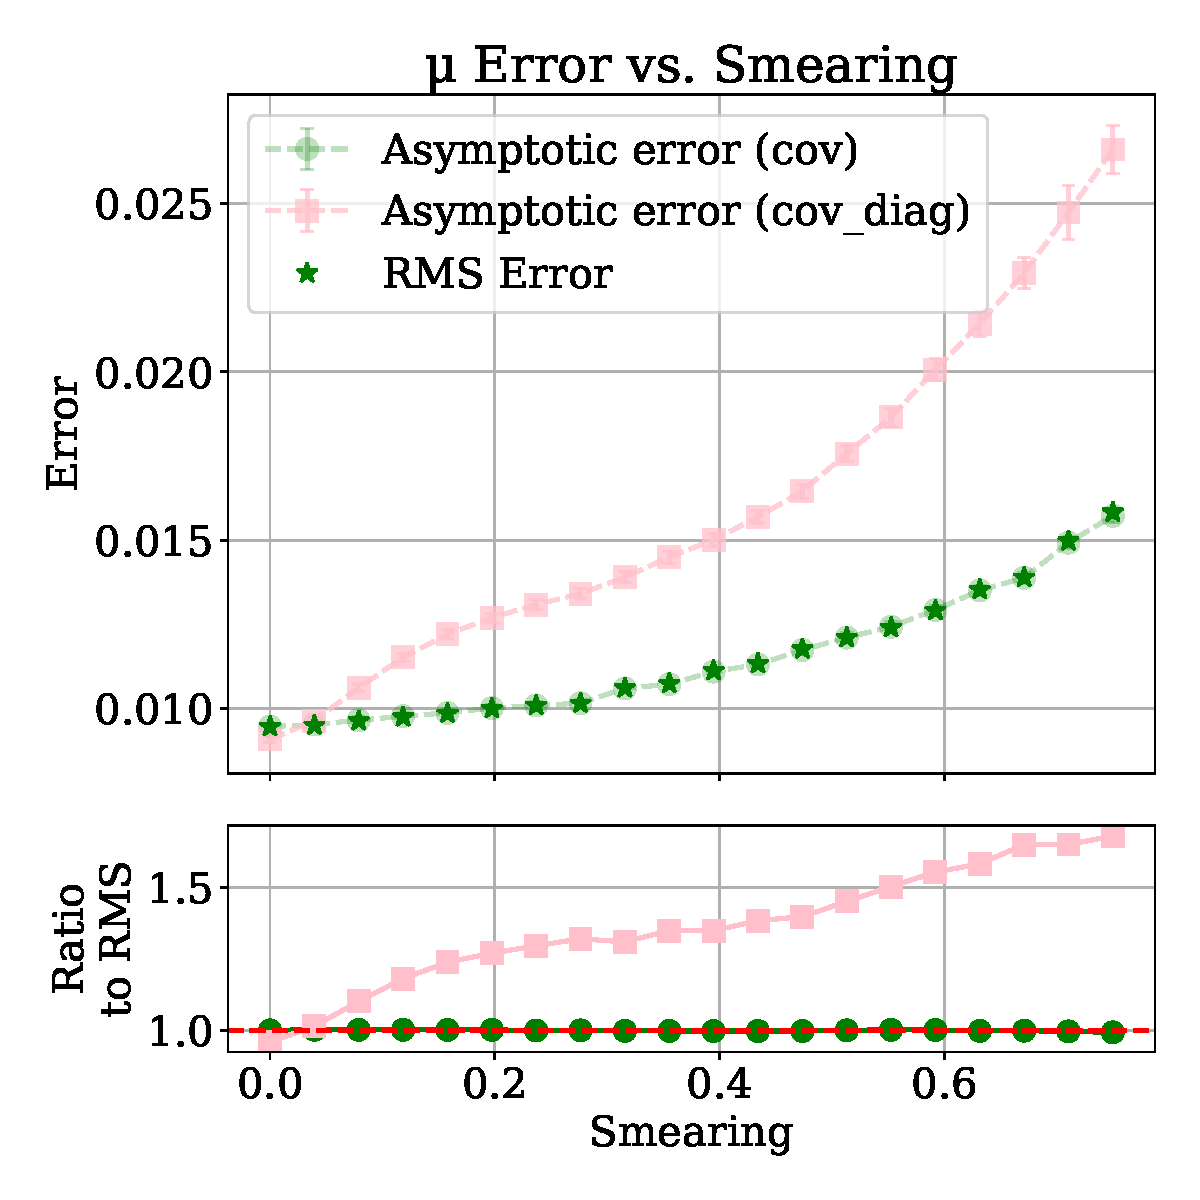
\includegraphics[width=0.43\linewidth]{figures/mu_error_plot_with_errorbars_ratio.pdf}
                \label{fig:mu_error_plot_with_errorbars}}\quad
                \subfloat[]{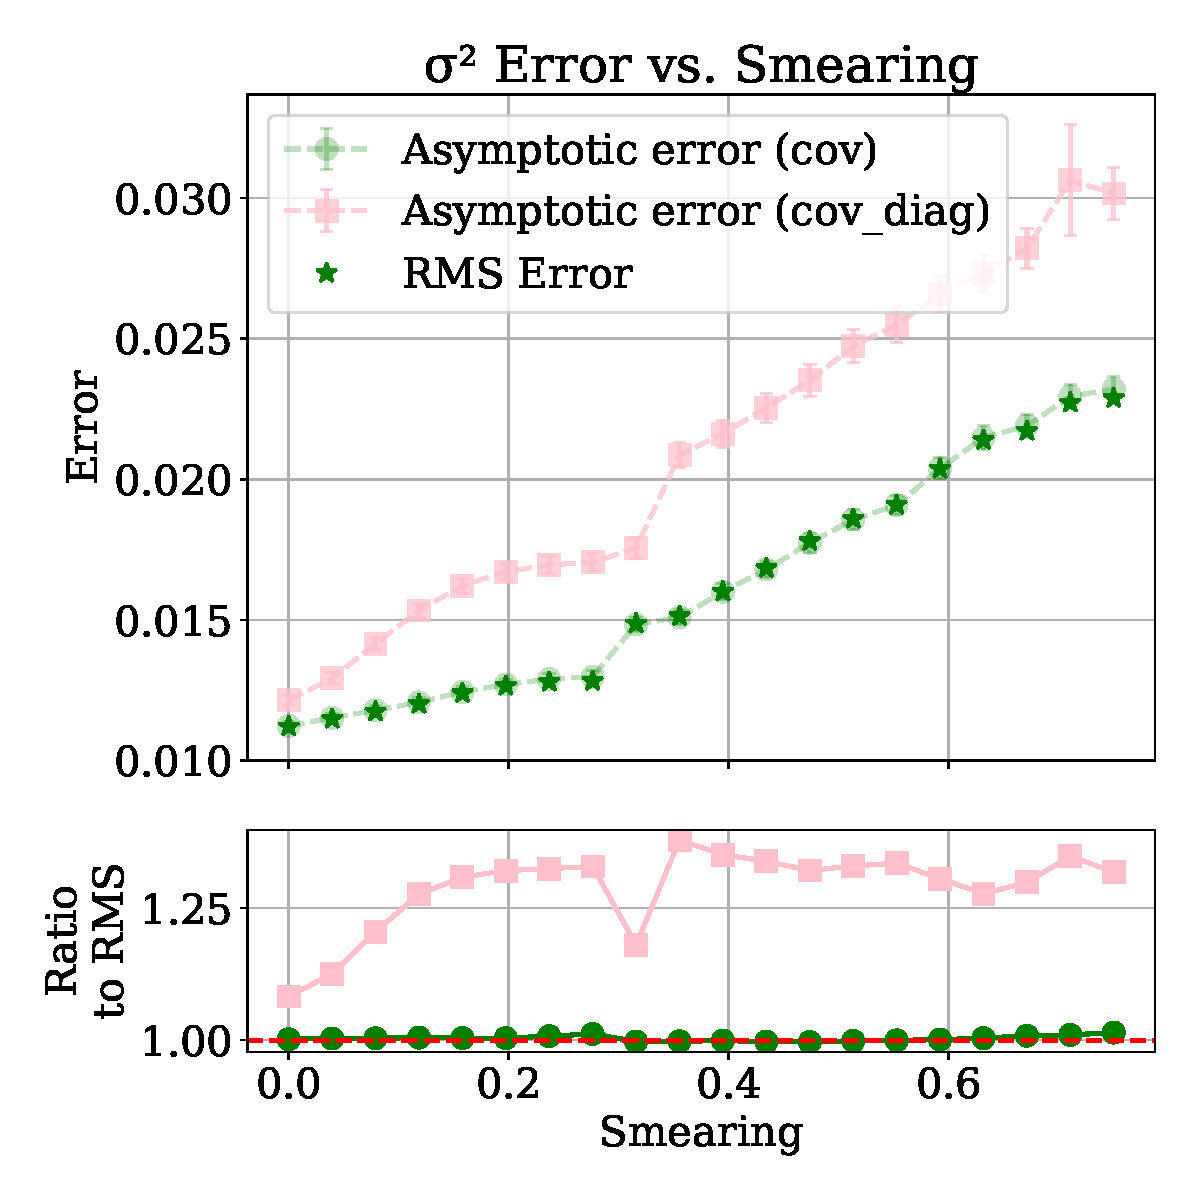
\includegraphics[width=0.45\linewidth]{figures/var_error_plot_with_errorbars_ratio.pdf}
                \label{fig:var_error_plot_with_errorbars}}
                \caption{Mean asymptotic \(1\sigma\) error versus detector smearing for the Gaussian (a) mean $\mu$ and (b) variance $\sigma^2$.
                %
                Results are shown for fits using the full covariance matrix (green circle markers) and using only the diagonal elements of the covariance (pink square markers).
                %
                The green stars represent the ``true" uncertainty determined by the standard deviation of the 500 fitted values from pseudo-experiments.
                %
                Observe that the asymptotic errors from the full--covariance fits agree very well with the ensemble spread (green circles overlapping green stars), while the diagonal--only approximation consistently overestimates the uncertainties, especially at larger smearing values (pink squares lie above the green stars).}
            \label{fig:uncertsfullybinned}
        \end{figure}
        \begin{figure}
            \centering
            \subfloat[]{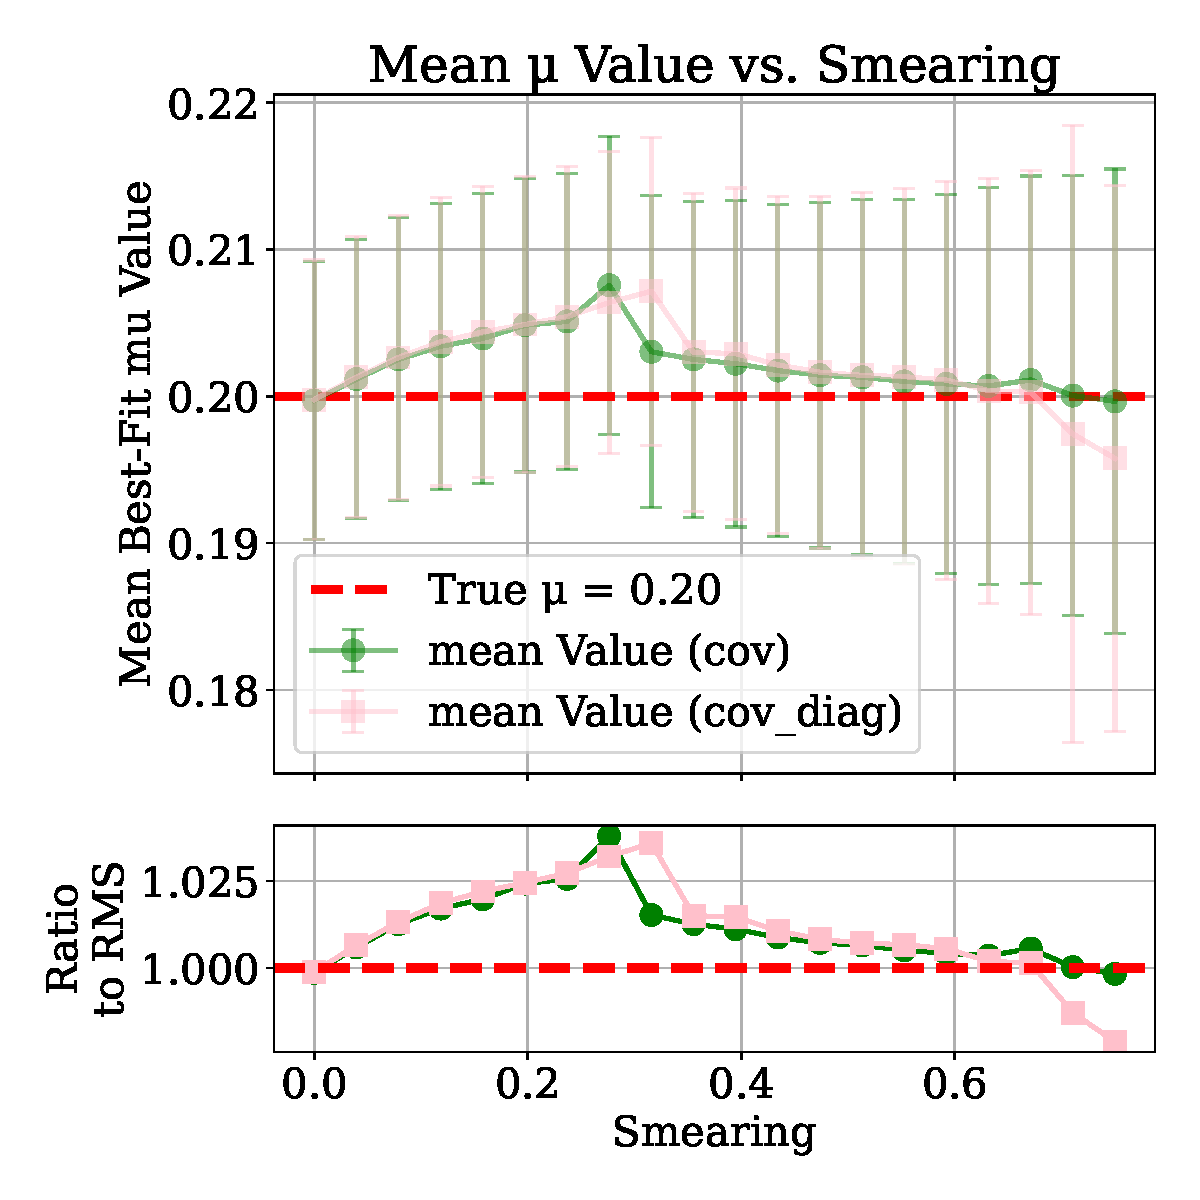
\includegraphics[width=0.43\linewidth]{figures/mu_mean_values_with_errorbars_ratio.pdf}
            \label{fig:mu_mean_values_with_errorbars}}\quad
            \subfloat[]{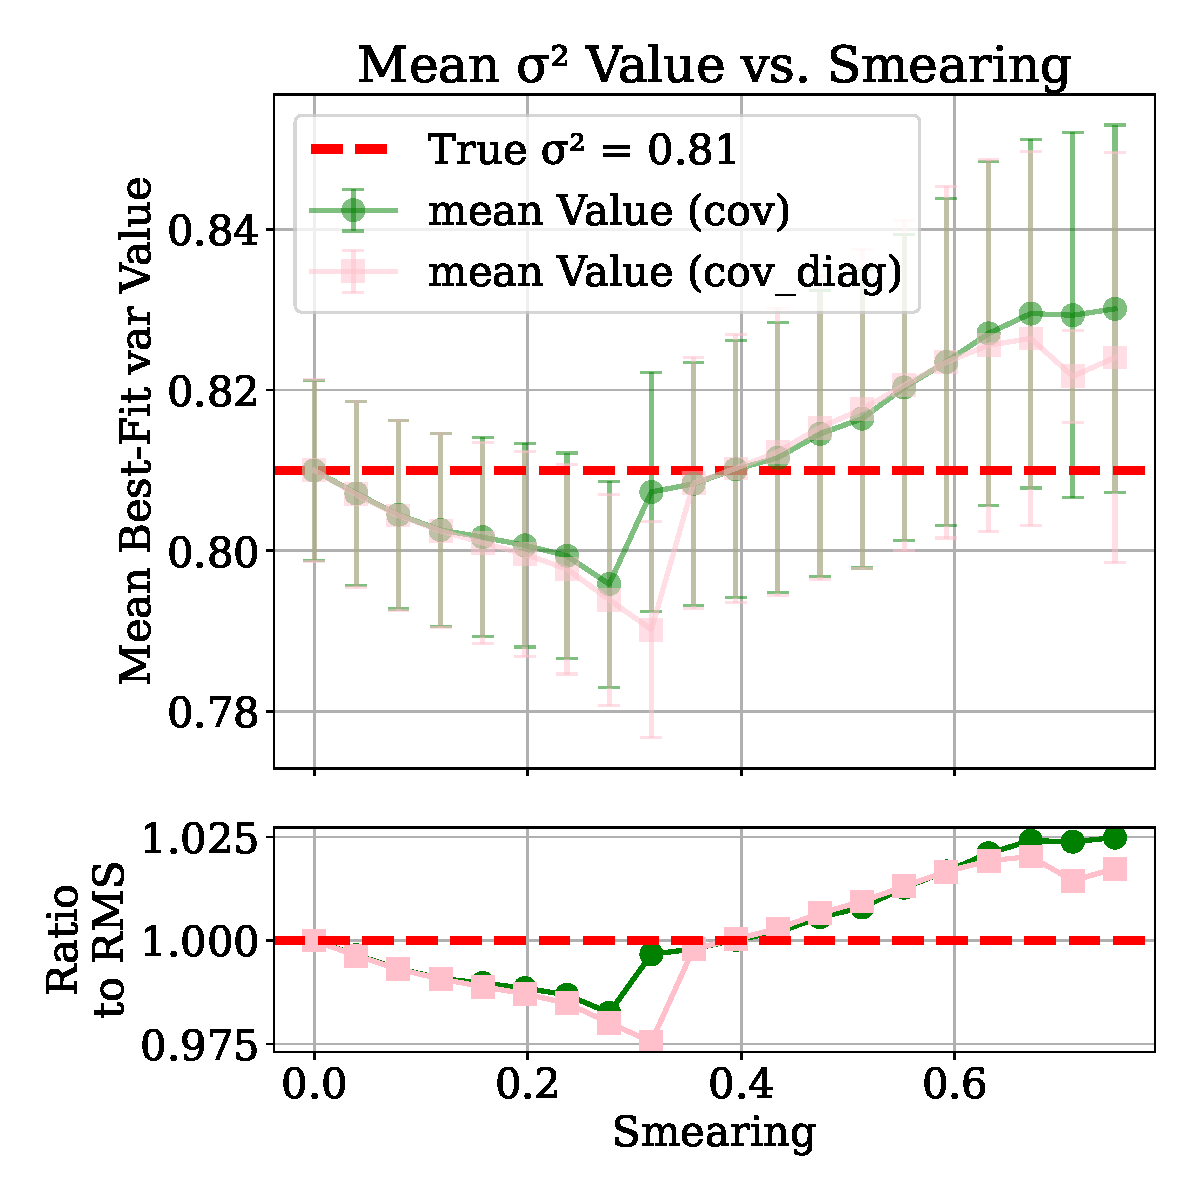
\includegraphics[width=0.43\linewidth]{figures/var_mean_values_with_errorbars_ratio.pdf}
            \label{fig:var_mean_values_with_errorbars}}
            \caption{
                The mean best-fit value of the Gaussian (a) $\mu$ and (b) $\sigma^2$ as a function of the detector smearing.
                % 
                Each point represents the average fitted value over 500 pseudo-experiments, with error bars showing the standard error on the mean (SEM).
                %
                The horizontal dashed red lines indicate the true parameter values ($\mu_{\text true}=0.2$ and $\sigma^2_{\text true}=0.81$).
                %
                Both fitting methods, using the full unfolded covariance (green circles) and using only diagonal uncertainties (pink squares), yield valid central values, demonstrating that the unfolding procedure is unbiased.
            }
        \end{figure}
    
        In summary, this study in the fully binned regime demonstrates that a conventional unfolding approach (IBU) combined with rigorous statistical treatment produces unbiased and well--calibrated inference of physics parameters.
        %
        The unfolded results, when analysed with their full covariance matrix, give parameter estimates whose uncertainties accurately reflect the true spread across experiments, ensuring correct confidence interval coverage.
        %
        We also see that simplifying assumptions like treating unfolded bins as independent can skew the uncertainty estimates, in this case, making them overly conservative, even though the point estimates remain correct.
        %
        These findings provide a critical baseline for comparison with the unbinned methods discussed in the next sections.
        %
        In the following section, we will investigate how unbinned unfolding techniques handle event correlations and whether they can achieve a similar level of statistical reliability as this fully binned approach. The lessons learned here, particularly the necessity of accounting for induced correlations, will carry forward as we transition to unbinned inference on correlated data.
    \subsection{Correlation Diagnostics after Unbinned Unfolding}
    \label{subsec:weight_correlations}
        Before confronting any inference procedure with an unbinned output, we must first quantify the statistical dependencies that the unfolding induces.
        %
        This subsection introduces two complementary diagnostics that make those correlations both {visible} and {quantifiable}.
        \begin{enumerate}
            \item the \textbf{pairwise weight–-distance correlation} $\rho(|x_i-x_j|)$ between all pairs unfolded events $i$ and $j$, and
            \item the \textbf{bin--bin covariance matrix} $C_{ab} = \operatorname{Cov}[\,\vb*{\nu}_a,\vb*{\nu}_b\,]$ of a fine histogram binned {after} unfolding.
        \end{enumerate}
        Both are evaluated for four detector resolutions $\sigma_{\det}\in\{0,0.25,0.50,0.75\}$ and for two distinct estimators, {KDE} and neural network (\textsc{NN}) conditional density estimators.
        %
        The results are displayed in \cref{fig:weight-corr} and \cref{fig:hist-cov}, respectively, and form the empirical basis for the coverage study in \cref{subsec:unbinned_data}.
        \subsubsection{Pairwise weight–-distance correlations}
        For every event, by considering the weight distributions across pseudo–-experiments one can compute the correlation coefficient, defined as
        \[
            \rho_{ij} = \frac{\mathrm{Cov}(w_i,w_j)}{\sigma_{w_i}\,\sigma_{w_j}}]
        \]
        One can then average $\rho_{ij}$ in bins of $\Delta x = |x_i-x_j|$, where $x$ is the unfolded observable.\footnote{
            %
            The average is taken after combining results from 500 pseudo–experiments; error bars in \cref{fig:weight-corr} denote the ensemble {RMS} of $\rho_{ij}$ in each $\Delta x$ bin, thereby incorporating both the statistical fluctuation correlations and any run-‐to-‐run variability of the unfolding.
            }
            %
            A few different features of the resulting curves (upper panels for {KDE}, lower for {NN}) are worth nothing.
            \begin{itemize}
            \item \emph{Perfect detector ($\sigma_{\det}=0$):}
                %
                One should expect the average pair-–wise correlation to be $\rho(|\Delta x|)\!\simeq\!0$ for all separations $\Delta x>0$, confirming that when no smearing is applied, \textsc{OmniFold} reproduces the {factorised likelihood} limit in which event weights are statistically independent\kd{cite:Andreassen:2019cjw}.
                %
                At $\Delta x = 0$ we trivially should expect $\rho(0)=1$ because every event is, of course, perfectly correlated with itself, and this is indeed what \cref{fig:weight-corr} demonstrates too.
                %
                In the truly ideal i.i.d. case, one would expect the fall off from $\rho(0)=1$ to $\rho(|\Delta  x|>0)\!=\!0$ to resemble a Dirac $\delta$ at the origin.
                %
                The {KDE} estimator indeed approaches this limit.
                %
                Its kernel bandwidth determines a correlation length \(\ell \lesssim\!0.15\).\kd{cite:Wasserman2006, WandJones1995}.
                %
                By contrast, even with extensive experimentation with architecture and hyperparameter tuning we find that {NN} priors leave a residual plateau $\rho\!\approx\!$\,$0.75$ around $\ell\!\approx\!1$, which then leads to the damped oscillatory structure of the correlation curve.
                %
                One could speculate about reasons why unfolding with neural networks even in the perfect detector resolution case should lead to correlated weights.
                %
                I propose two potential explanations.
                \begin{enumerate}
                    \item \emph{Network smoothness:} the shared weights in the neural network classifier impose a finite ``receptive field, \kd{cite:Minderer2021SmoothNN,WeightConditioning2024} causing nearby events to receive similar gradient updates and hence correlated weights; and
                    \item \emph{Global normalisation:} \textsc{OmniFold} enforces $\sum_i w_i = N_{\text{MC}}$ at every iteration.
                    %
                    This normalization might be introducing a weak positive correlation of size $1/N$ even in the absence of detector effects\kd{cite:Cowan2011Stats}. 
                \end{enumerate}
                Although numerically tiny, this effect, whatever its underlying explanation sets the optimistic lower bound on variance reduction when working with neural networks.
                %
                Thus even the idealised zero--smearing case does not yield {perfectly} independent weights in practice, a useful caution when quoting statistical uncertainties from inference using ML processed data.
            \item \emph{Mild smearing (\(\sigma_{\det}=0.25\)):}
                %
                Short--range correlations of order \(\rho\gtrsim 0.5\) appear for \(\Delta x\lesssim0.4\).
                %
                These are already sufficient to reduce the {effective sample size}
                \[
                  N_{\text{eff}} = N/\!\bigl[\,1+(N-1)\rho\bigr]
                  \]
                  \kd{cite} considerably.
                  %
                  \(\rho < 0\) for \(\Delta \in [1, 2]\), as expected.
                  %
                  For both the NN and the KDE, \(\rho\) exhibits the same damped oscillatory structure, as would be expected by the normalization imposed by the unfolding.
                  %
                  \(\ell_{\text{KDE}}\) is noticeably smaller that \(\ell_{\text NN}\).
                  %
                  The contrast is less pronounced than in the perfect-resolution case, yet still visible.
            \item \emph{Moderate and large smearing ($\sigma_{\det}\ge0.5$):}
                % 
                Correlations develop a broad plateau {independent of distance}.
                %
                In that regime $N_\text{eff}$ collapses explaining why a naïve fit ignoring  correlations would significantly misestimate errors.
            \end{itemize}
            The \textsc{NN} generally yields more long range, but {slightly weaker} correlations than the \textsc{KDE} at the same resolution, suggesting that a higher-‐capacity estimator might be able to better absorb detector noise. 
            %
            However, the qualitative behaviour is identical;
            any non–zero smearing produces, long‐range weight correlations that violate the i.i.d. assumption built into standard unbinned likelihoods\kd{cite}.
        \subsubsection{Histogram covariance matrices.}
            Since most downstream analyses eventually bin the unfolded events, a histogram covariance matrix can be effective to visualize the correlations.
            %
            To visualise the impact on such \emph{binned} summaries we fill a 40‐bin histogram in the range $[-4,4]$ for each pseudo–experiment and compute
            \[
              C_{ab} = \bigl\langle
                         (N_a-\bar N_a)(N_b-\bar N_b)
                       \bigr\rangle.
            \]
            %
            The matrices, shown in Fig.~\kd{fig:hist-cov}, reinforce the observations from the correlation curves.
            %
            Even at zero smearing, while KDE produces a nearly diagonal $C_{ab},$ \textsc{OmniFold}'s weights exhibit small but noticable off diagonal elements.
            %
            Growing the smearing leads to pronounced \emph{anti-‐correlations} along the first off–-diagonal and coherent positive correlations far from the diagonal.
            %
            For $\sigma_{\det}=0.75$ the largest off–diagonal coefficient reaches $|\rho_{ab}|\simeq0.5$, echoing the plateau seen in $\rho(|\Delta x|)$.  These patterns are almost identical for {KDE} and {NN} analyses.

            Such strong off–-diagonal structure rigorously explains why a $\chi^2$ fit that {ignores} covariances by using only the diagonal of $C$ leads to miscoverage.
        \subsubsection{Implications}
            The correlation diagnostics presented here {empirically validate} the theoretical expectation that \textsc{OmniFold} weights are correlated.
            %
            Quantifying the strength and range of those correlations enables an \emph{a priori} estimate of how badly an independence‐-based error formula will fail\kd{cite}.
            %
            They provide {input templates} and motivation for developing a rigorous covariance‐aware asymptotic method.
            %
            With these diagnostics in hand, we are now equipped to benchmark the statistical performance of binned and unbinned inference workflows on unbinned unfolded data, which is the subject of the next subsection.
    \subsection{Unbinned Unfolding: Binned and Unbinned Inference}
    \label{subsec:unbinned_data}
        Having established a fully binned baseline in the previous section, we now examine two inference workflows that utilize unbinned unfolding on the same Gaussian data.
        %
        Both approaches start by unfolding the detector--level data without binning, producing a set of weighted events at truth--level.
        %
        Because the deconvolution process induces non--negligible correlations between event weights (especially for finite detector smearing, as evidenced by the covariance patterns in \cref{fig:weight-histogram-covariance-1d}), these workflows differ in how they handle those correlations.
    
        When performing binned inference on unbinned unfolded data, the unfolded weighted events are aggregated into a histogram, and a binned template fit is performed using a $\chi^2$ statistic that includes the full binned covariance matrix.
        %
        In these experiments, the unfolded distribution is fit to the parametric Gaussian model (with mean $\mu$ and variance $\sigma^2$) by integrating the model prediction over the histogram bins.
        %
        The covariance matrix of the bins is estimated from an ensemble of repeated pseudo--experiments.
        %
        One then obtains best fit parameters by $\chi^2$ minimization and determines their uncertainties via the usual $\Delta\chi^2=1$ criterion.
        %
        This approach is analogous to a standard binned analysis except that the data have been unfolded using an unbinned method.
        %
        Crucially, it retains statistical rigour by propagating the full unfolding--induced covariance into the fit.
    
        Alternatively, one could attempt to fit the parametric model directly to the weighted events using an unbinned maximum--likelihood procedure that ignores inter--event correlations.
        %
        One constructs the negative log likelihood,
        \[
            \operatorname{NLL}(\theta) = -\sum_{i=1}^N w_i \ln P(x_i \mid \theta),
        \]
        where $x_i$ and $w_i$ are the kinematic value and weight of event $i$, and $P(x_i|\theta)$ is the model density for parameters $\theta=(\mu,\sigma^2)$.
        %
        This unbinned likelihood sum is maximized to obtain the best fit $\hat\theta$.
        %
        The Hessian (curvature) of the NLL at the optimum provides an asymptotic error estimate for $\theta$.
        %
        Equivalently, one finds the $\Delta\ln L=0.5$ offset for a $1\sigma$ interval.
        %
        This workflow assumes statistical independence of events.\kd{cite:Cowan:2002in,Blobel:2203257}.
        %
        Thus, while method the latter method yields a fit and a formal error bar, these must be interpreted with caution since the underlying likelihood model is misspecified.
    
        Both of the above approaches are applied to the same Gaussian datasets described earlier in \cref{subsec:setup}.
        %
        Unfolding is performed with the \textsc{OmniFold} algorithm\kd{cite:Andreassen:2019cjw,Andreassen:2021zzk}.
        %
        In the one dimensional setting we also test a KDE based implementation.
        %
        For each resolution setting, the 500 pseudo--data samples are unfolded and then subjected to both the aforementioned inference procedures.
        %
        This allows us to compare the bias, uncertainty estimation, and coverage of the two workflows against the fully binned baseline.
        \paragraph{Parameter Bias}
            Both unbinned workflows yield fitted parameter values that are consistent with those from the binned baseline.
            %
            In fact, we find no appreciable additional bias introduced by the unbinned unfolding step or the choice of inference method.
            %
            \cref{fig:uncertainty-and-bias-vs-resolution} (bottom panels) shows the mean fitted $\mu$ and $\sigma^2$ as a function of detector smearing for each method.
            %
            All approaches produce estimates of $\mu$ and $\sigma^2$ across the range of smearings within the statistical uncertainties.
            %
            Notably, the bias observed in the naive unbinned ML fit is the same as that in the proper $\chi^2$ fit that accounts for the covariance of a given dataset. 
            %
            This can be explained as both fits ultimately maximizing a likelihood (or minimizing a $\chi^2$) to match the unfolded distribution to the model;
            %
            if the model is correctly specified, the MLEs should coincide.
            %
            Thus, unbinned unfolding does not itself induce a bias in the extracted physics parameters verifying the claim that the \textsc{OmniFold} procedure (with sufficient iterations and regularization) correctly reproduces the shape of the true distribution on average.\kd{cite:Andreassen:2019cjw}
            %
            This is demonstrated by the agreement of fitted values with the true parameter shown by the horizontal lines in Fig.\cref{fig:uncertainty-and-bias-vs-resolution} and the baseline results in \cref{fig:mu_mean_values_with_errorbars}. 
        \paragraph{Uncertainty estimation and coverage}
            In sharp contrast to the agreement in central values, the two workflows differ markedly in their reported uncertainties and the statistical coverage of those uncertainties.
            %
            The binned-$\chi^2$ approach with full covariance proves to be consistent with the baseline in its uncertainty estimates.
            %
            For each smearing level, the asymptotic $1\sigma$ errors obtained from the $\Delta\chi^2=1$ criterion agree well with the empirical spread (RMS) of the fitted parameters over the 500 pseudo-experiments.
            %
            This is illustrated in the top panels of \cref{fig:uncertainty-and-bias-vs-resolution}: the curve corresponding to the full-covariance $\chi^2$ fit lies on top of the true uncertainty obtained from the pseudo-data ensemble (star markers), for both $\mu$ (left) and $\sigma^2$ (right). In other words, binned inference on unbinned data using a \(\chi^2\) fit that incorporates the full covariance matrix produces accurate confidence intervals that maintain the nominal coverage.
            %
            This behaviour is as expected and desired.
            %
            By incorporating the complete covariance matrix of the unfolded histogram, we correctly account for the event correlations in the statistical inference.
            %
            Indeed, these results mirror the fully binned study.
            %
            Recall that in the baseline binned analysis, using the full covariance matrix yielded uncertainty estimates consistent with the bootstrap pseudo--data spread, whereas using only diagonal uncertainties did not, as shown in \cref{fig:uncertsfullybinned}.
            %
            We explicitly confirm the same result in the unbinned case too.
            %
            If one performs a binned fit to the unfolded histogram but (incorrectly) ignores off--diagonal bin correlations, the uncertainties are overestimated and the $\chi^2$ fit yields unnecessarily large error bars, analogous to the diagonal--covariance points in \cref{fig:uncertsfullybinned}.
            %
            This over--conservative result similarly arises from double--counting the anti--correlated fluctuations in each bin and leads to overcoverage, further underscoring that the full covariance is essential for a proper statistical treatment .
    
            By contrast, the naïve unbinned ML inference on the unbinned data fails to produce correct uncertainty estimates.
            %
            As shown in \cref{fig:uncertainty-and-bias-vs-resolution} (top panels, orange points), the asymptotic errors reported by the unbinned likelihood fit are dramatically smaller than the true spread of the fit results, except in the trivial case of zero smearing.
            %
            Intriguingly, the naive unbinned error bars hardly change with detector resolution---the orange curve in \cref{fig:uncertainty-and-bias-vs-resolution} is nearly flat---indicating that the fit is seemingly just as ``precise" for a very smeared dataset as for a perfect detector.
            %
            This unphysical result is a direct consequence of ignoring the event correlations.
            %
            The ML fit treats each weighted event as independent information, thereby overestimating the effective sample size.
            %
            Intuitively, when events are strongly correlated, the true number of independent degrees of freedom is smaller than $N$; but the naive NLL sum scales like $N$, yielding an misestimate of the variance of $\hat\theta$.
            %
            In our Gaussian example, the effect is severe even at moderate smearing.
            %
            For instance, at $\sigma_{\text det}=0.5$ the unbinned ML formula underestimates the uncertainty on $\mu$ by roughly a factor of two compared to the bootstrap truth, and at $\sigma_{\text det}=0.75$ the discrepancy is even larger.
            %
            This breakdown of the asymptotic approximation in the presence of inter--event correlations is the essential failure mode of the naive unbinned approach.
            %
            It should be emphasized that when the detector resolution is perfect (no smearing), the unfolding induces no correlations and indeed the unbinned ML errors do coincide with the correct uncertainties, and all methods become equivalent in this limit.
            %
            But for any non--zero smearing, the independence assumption is violated and the standard likelihood formulae no longer hold.
            %
            The unbinned fit still finds the correct central values, but its error estimates must not be trusted.
    
        The practical implication of these findings is that naively applying unbinned inference to unfolded data can produce misleadingly constraints, even though the fit may appear to converge normally.
        %
        In our study, the na\"ive unbinned workflow would have erroneously suggested measurement insensitive to detector smearing, whereas in truth the uncertainties should grow with smearing, as correctly reflected by methods that account for correlations.
        %
        This highlights the necessity of handling the event correlations in some way, potentially through the hybrid approach.
        %
        By introducing a binning at the final inference stage and using a covariance matrix, one essentially restores statistical consistency, at limits the impact of binning artifacts.
        %
        Such an approach largely retains the benefits of unbinned unfolding, with no information loss up to the point of inference, while yielding parameter uncertainties and coverage properties in line with a rigorous frequentist construction.
        %
        Hence this ``unbinned unfolding + binned fit'' should be more precise than a fully binned analysis.
        %
        For example, in \cref{fig:uncertainty-and-bias-vs-resolution} the full covariance UBU results achieve a similar or smaller uncertainty than the traditional IBU based results at each smearing value.
        %
        This suggests an advantage to delaying any binning as late in the analysis chain as possible, consistent with the intuition that using unbinned distributions throughout the unfolding can preserve more information for the final fit\kd{cite:Andreassen:2019cjw}.
        %
        One should note, however, that in the 1D case this advantage is modest.
        %
        UBU and IBU approaches do not differ vastly in precision.
        %
        In higher dimensions the unbinned approach is expected to drastically outperform a binned analysis (since binning in many dimensions is impractical or introduces large discretization errors)\kd{cite:Pan:2024rfh,Butter:2022rso2}.
    
        While the hybrid method provides a sound stopgap, it somewhat undermines the original motivation for unbinned methods, which aimed to avoid histogramming altogether.
        %
        The fully unbinned method, on the other hand, fully actualizes the principle underlying the unbinned paradigm but lacks a statistical asymptotic formalism that accounts for correlations.
        %
        The stark miscoverage we observe for the naive unbinned fit underlines the need for correlation--aware unbinned inference techniques.
        %
        In other words, if one wishes to perform event--level likelihood fits on unfolded data, one must either develop a formalism to incorporate the event--to--event covariance information into the likelihood or rely on numerical methods to calibrate the uncertainties.
        %
        In this study, one does finds that if one estimates uncertainties numerically through pseudo--experiments or bootstraps, the precision of the unbinned fit can be evaluated correctly.
        %
        This is evidenced by the fact that the RMS spread of the naive ML fit outcomes (the blue line in \cref{fig:uncertainty-and-bias-vs-resolution}) does increase with smearing and matches the covariance-fit results.
        %
        However, using brute force pseudo--experiments or bootstraps to determine errors is computationally expensive and may not be feasible in a real experiment.
        %
        Besides, errors computer through bootstrapping offer no analytical understanding of the uncertainty.
        %
        Nonetheless, until a theoretical framework is developed to handle correlations at the likelihood level, any unbinned inference on unfolded events should be performed through bootstrapping.
    
        In summary, the comparison of binned versus unbinned inference after unbinned unfolding reveals that both workflows yield unbiased parameter estimates, but only the approaches that account for correlations produces reliable uncertainties and coverage.
        %
        A na\"ive approach of treating weighted unfolded events as independent leads to misestimated uncertainties and hence significant miscoverage.
        %
        These results vividly demonstrate the statistical pitfalls of ignoring induced correlations, and they motivate the correlation--aware inference strategies discussed in the next section.
        %
        As unbinned unfolding techniques become increasingly prevalent in extracting cross sections\kd{cite:ATLAS:2024xxl,ATLAS:2025qtv,CMS-PAS-SMP-23-008}, developing a robust framework to correctly propagate uncertainties through the unbinned pipeline is essential.
        %
        This study provides a first quantitative glimpse of the issue, showing that while unbinned unfolding can preserve accuracy and potentially improve precision, one must incorporate the full correlation structure to achieve valid statistical inference.
        %
        This will be crucial for ensuring proper coverage and trustworthy uncertainty estimates in future high--dimensional unfolding analyses.
    \subsection{Extension to Higher Dimensions}
    \label{sec:highD_extension}
        The diagnostics of \cref{subsec:weight_correlations,subsec:unbinned_data} established that even in {one} dimension the naïve unbinned likelihood approach
        seriously underestimates uncertainties once unfolding procedure induces correlated event weights.
        %
        A natural next question is whether that pathology grows, diminishes, or saturates as one moves to multi–-differential measurements.
        %
        We therefore repeat the Gaussian study in two, four and six dimensions, keeping the experimental setup identical, except for adjusting the numerical parameters that define the Gaussians.
        %
        The Gaussian parameters used in the multidimensional studies are listed in \cref{tab:highD-params}.
        %
        Detector resolutions are scaled coordinate--wise so that the signal‐-to-‐noise ratio in every dimension matches the 1--D baseline.
        \begin{table}
            \centering
             \caption[Gaussian model parameters for multidimensional studies]{
                Gaussian parameters used in the \(2, 4\), and \(6-\)dimensional toy studies.
                %
                The column vectors \(\boldsymbol{\mu}\) and \(\boldsymbol{\sigma}\) list the component means and standard deviations, respectively.
                %
                \(\rho\) denotes the linear correlation matrix.
                %
                Detector resolutions \(\boldsymbol{\sigma}_{\det}\) are applied component-wise as additive Gaussian noise in the detector simulation.
                }
            \label{tab:highD-params}
            \scriptsize
            \begin{tabular}{M M M M}
              \toprule
            & \textbf{Gen.} & \textbf{Det.}& \textbf{Truth}\\
              \midrule
              && \textbf{2--D}\\
                 \vb*{\mu}  & \mqty[0.0\\1.0]  && \mqty[0.2\\0.8]\\[16pt]
              \boldsymbol{\sigma}        & \mqty[1.0\\1.5]                     & \mqty[0.5\\0.8]& \mqty[0.9\\1.3]\\[16pt]
              \rho                       & \mqty[1.0 & -0.6 \\ -0.6 &  1.0]    && \mqty[1.0 & -0.6 \\ -0.6 &  1.0]\\
              \midrule
              
              && \textbf{4--D}\\
              \vb*{\mu}                  & \mqty[1.0\\0.0\\-0.5\\0.5]          && \mqty[0.8\\0.1\\-0.6\\0.7]\\[16pt]
              \boldsymbol{\sigma}        & \mqty[1.0\\0.7\\1.1\\0.8]           &\mqty[0.4\\0.5\\0.6\\0.3]& \mqty[0.8\\0.6\\1.0\\0.6]\\[16pt]
              \rho & \mqty[
                       1.0 &  0.1 & -0.2 &  0.3\\
                       0.1 &  1.0 &  0.0 &  0.1\\
                      -0.2 &  0.0 &  1.0 &  0.7\\
                       0.3 &  0.1 &  0.7 &  1.0] &&
                    \mqty[
                       1.0 &  0.0 & -0.3 &  0.4\\
                       0.0 &  1.0 &  0.2 &  0.0\\
                      -0.3 &  0.2 &  1.0 &  0.5\\
                       0.4 &  0.0 &  0.5 &  1.0]\\
              \midrule
              
              &&\textbf{6--D}&\\
              \vb*{\mu}                  & \mqty[ 1.0\\ 0.0\\-0.5\\ 0.5\\-1.0\\ 0.3] &&
                                            \mqty[ 0.8\\ 0.1\\-0.6\\ 0.7\\-0.8\\ 0.1]\\[16pt]
              \boldsymbol{\sigma}        & \mqty[ 1.0\\ 0.7\\ 1.1\\ 0.8\\ 1.2\\ 1.4] & \mqty[0.4\\0.5\\0.6\\0.3\\0.4\\0.4]
              & \mqty[ 0.8\\ 0.6\\ 1.0\\ 0.6\\ 1.0\\ 1.1]\\[16pt]
              \rho & \mqty[
                       1.0 &  0.1 &  0.2 & -0.3 &  0.0 &  0.0\\
                       0.1 &  1.0 &  0.0 & -0.2 &  0.3 &  0.1\\
                       0.2 &  0.0 &  1.0 &  0.1 & -0.2 &  0.3\\
                      -0.3 & -0.2 &  0.1 &  1.0 &  0.1 &  0.0\\
                       0.0 &  0.3 & -0.2 &  0.1 &  1.0 &  0.7\\
                       0.0 &  0.1 &  0.3 &  0.0 &  0.7 &  1.0] &&
                    \mqty[
                       1.0 &  0.0 &  0.2 & -0.2 &  0.1 &  0.0\\
                       0.0 &  1.0 &  0.0 & -0.1 &  0.2 &  0.0\\
                       0.2 &  0.0 &  1.0 &  0.0 & -0.3 &  0.4\\
                      -0.2 & -0.1 &  0.0 &  1.0 &  0.2 &  0.0\\
                       0.0 &  0.2 & -0.3 &  0.2 &  1.0 &  0.5\\
                       0.0 &  0.0 &  0.4 &  0.0 &  0.5 &  1.0]\\
              \bottomrule
            \end{tabular}
        \end{table}
        \subsubsection{Evaluation}
            For every fit parameter (all $\mu_k$ and all unique $\sigma^2_{kl}$) we compute the {empirical RMS} over 500 pseudo-–experiments, and the average asymptotic error reported by the naïve unbinned–likelihood Hessian.
            %
            If the likelihood were well–-calibrated, these two quantities
            should coincide.
            %
            \cref{fig:rms-asy-dim} plots RMS versus asymptotic error for all parameters in 1, 2, 4, and 6--D.
            %
            The dashed diagonal marks perfect agreement and the solid green line has a slope fixed to the mean of the RMS/asymptotic‐-error ratio for that dimension.
            
            As we can see, in each case, the RMS uncertainty is higher than the asymptotic uncertainty.
            %
            The ratio of the RMS uncertainty to the asymptotic uncertainty is roughly the same for all of the model parameters with the ratio ranging from 1.18 to 1.28.
            %
            The analytic error bars understate the true variance by a factor $\sim\!3$–4, consistent with the effective sample size argument.\kd{https://andrewcharlesjones.github.io/journal/21-effective-sample-size.html}.
            
            \cref{fig:rms-asy-6D-res} repeats the 6--D study with detector resolution scaled by $0,1,2,$ and $3$ relative to the $\sigma_{\det}$ in \cref{tab:highD-params}.
            %
            The slope grows with the smearing factor, confirming that weight correlations, not intrinsic variance, drive the failure\kd{Eur. Phys. J. C 82 (2022) 393}.

            In high dimensions, the mapped weight vector $w(\mathbf{x})$ is a smooth function on a space where almost all pairs of points are distant.
            %
            Hence the classifier must assign similar gradients to a larger neighbourhood, inflating correlations.
            %
            \kd{https://aicompetence.org/kernel-density-estimation-non-parametric-probability/} explains this phenomenon for KDEs, where excessively wide kernels force longer--range weight correlations.
            %
            The same effect applies to NNs as well because global normalisation $\sum_i w_i=N_{\text{MC}}$ adds an $\mathcal O(1/N)$ positive correlation to {every} pair of events\kd{PhysRevD.90.072004}.

            In six dimensions the naïve asymptotic formula would underestimate statistical errors for several covariance elements, while the RMS spread shows true uncertainties.
            %
            For collider analyses, where multi-differential analyses are the future, this degree of systematic undercoverage is unacceptable.
            %
            Either a binned-covariance approach  or a correlation-aware unbinned likelihood\kd{https://indico.cern.ch/event/671301/contributions/2745801/attachments/1557488/2449991/171113-unfold.pdf} is necessary.
            %
            Recent proposals such as Schrödinger--bridge unfolding\kd{arxiv 2308.12351}, or low-rank covariance compression\kd{arXiv:1802.06048} offer interesting possibilities for exploration.
            \begin{figure}
                \centering
                \includegraphics[width=\linewidth]{figures/RMS_vs_Asy_AllDims.pdf}
                \caption{Scatter of empirical RMS vs. mean asymptotic uncertainty for every model parameter in 1, 2, 4 and 6--D unbinned unfolding studies.
                %
                The grey dashed line has unit slope; green line's slope equals the mean RMS/asymptotic ratio for that dimension.
                }
                \label{fig:rms-asy-dim}
            \end{figure}

            \begin{figure}[htbp]
                    \centering
                  \includegraphics[width=0.8\linewidth]{figures/RMS_vs_Asy_6D_SmearingScan.pdf}
                  \caption{Same as Fig.~\ref{fig:rms-asy-dim} but confined to the 6--D
                  study and showing four detector–smearing scale factors
                  ($0,1,2,3$).
                  %
                  Increased smearing increases correlations and drives the
                  RMS/asymptotic slope ever further above unity.
                  }
                  \label{fig:rms-asy-6D-res}
            \end{figure}
\section{Conclusions and Outlook}
    This chapter presented a detailed study of parameter inference performed on an unbinned unfolded dataset, using a controlled Gaussian simulation.
    %
    By employing a simplified scenario where the true distribution and detector response are known analytically, we were able to isolate and rigorously examine the statistical subtleties introduced by unbinned unfolding.
    %
    The Gaussian studies demonstrated that preserving event--level information until the final fit can indeed confer a tangible advantage: an unbinned unfolding followed by parameter estimation was observed to outperform a fully binned analysis in terms of fit precision.
    %
    This validates the intuitive principle that one should delay information reduction (e.g. binning) as much as possible in the analysis chain, thereby maximizing the use of available information.
    %
    Importantly, however, the findings also exposed critical caveats that must temper this optimism, especially when interpreting unbinned results with standard inference techniques.

    A central observation is that the output of an unfolding procedure violates the usual assumption of statistical independence among events.
    %
    In our studies, the iterative \textsc{OmniFold} procedure produces a weighted set of “unfolded” events that are correlated with one another.
    %
    We showed that a naïve unbinned likelihood--based inference, which treats the unfolded events as if they were independent observations, fails to yield reliable uncertainty estimates.
    %
    In particular, when event--to--event correlations are ignored, the standard asymptotic formulae for parameter uncertainties\footnote{derived from a Fisher information or Hessian approximation} become invalid.
    %
    Concretely, the naive application of an unbinned maximum likelihood fit dramatically underestimates the true uncertainty on the fitted parameters in Gaussian examples.
    %
    This underestimation was evidenced by comparing the analytic errors to the empirical spread of fit results across many pseudo-experiments.
    %
    The analytic errors, assuming independence, were significantly smaller than the actual RMS of the fitted parameters.
    %
    Such a discrepancy is a direct manifestation of ignoring the induced correlations and a clear warning that conventional inference tools cannot be blindly applied to unbinned unfolded data.
    %
    In short, the lack of statistical independence introduced by unbinned unfolding can invalidate classical error estimates, and thus the entire inferential procedure must be handled with care.

    On the positive side, the investigation also highlighted that correlation--aware approaches can effectively restore valid inference, albeit with practical limitations.
    %
    When one incorporates the inter--event correlations into the analysis, one finds that the derived uncertainties align with the true performance of the fit.
    %
    In the Gaussian studies, the numerically estimated uncertainties, obtained from the spread of outcomes over many trials, agree well with a covariance--informed analytical approach, confirming that the primary cause of the asymptotic formula breakdown was the neglect of correlations.
    %
    This serves as an important proof of principle.
    %
    If one properly accounts for the covariance between events\footnote{or equivalently, between event weights} in the unbinned dataset, inference methods can yield correct confidence intervals and hypothesis tests even in the unbinned paradigm.
    %
    However, it should also be emphasized that such covariance-aware treatments are computationally challenging to scale.
    %
    In a binned analysis the covariance matrix is of manageable size, but in an unbinned analysis even if a suitable covariance kernel, one in principle faces an $N \times N$ covariance among $N$ events or event weights, which is intractable for the large event samples typical of collider data.
    %
    The use of bootstrap ensembles to numerically evaluate uncertainties, while effective for a toy study, would be prohibitively expensive for high--dimensional or high--multiplicity data.
    %
    Thus, the practical implementation of correlation--aware unbinned inference encounters serious scaling limitations, underscoring the need for new strategies to handle or approximate these large covariance structures.

    Crucially, the results presented here should be viewed as a cautionary case study rather than a definitive statement on all unbinned analyses. 
    %
    They were obtained in an idealized Gaussian context, with complete knowledge of the generative process.
    %
    This controlled setup allows one to rigorously identify potential pitfalls and verify proposed solutions, but it also means that the qualitative behaviours observed might not universally translate to real collider data.
    %
    In particular, the observation that ignoring correlations had little impact on the central values and empirical precision of the fit in the Gaussian example may be a fortunate consequence of the symmetry and simplicity of that example.
    %
    One should not assume this will hold in general.
    %
    Therefore, while this study provides a rigorous proof of principle and important warnings, further work is required to generalize of these findings.
    %
    The takeaway is that we have uncovered a set of statistical issues that could plausibly afflict unbinned cross section measurements, and we have verified their existence in a controlled setting.
    %
    It now remains to investigate whether and how these issues manifest in realistic analyses.
    %
    This chapter’s findings should motivate vigilance so that any inference on unbinned unfolded data must be scrutinized for hidden correlations, and current methods must be extended before one can rely on them in full generality.

    Looking ahead, our work motivates several important future directions for both methodology and application.
    %
    An immediate next step is to extend these diagnostic studies to real collider observables and data.
    %
    It will be invaluable to apply similar techniques (e.g. pseudodata experiments, bootstrap uncertainty evaluations, and covariance measurements) to a realistic experimental unfolding scenario, for example, a differential cross section measurement published with unbinned results, to evaluate the size of event--level correlations and to quantify their impact on parameter fits.
    %
    Such studies on real or high fidelity simulated data would confirm whether the cautionary lessons from the Gaussian example are broadly applicable, and could reveal any additional complications arising from more complex data structure or detector effects.
    %
    Another critical line of research is to develop new statistical frameworks for unbinned inference that explicitly account for event correlations.
    %
    This could involve formulating modified likelihood functions or test statistics that include correlation terms, or designing hybrid approaches that retain the advantages of unbinned data while imposing an effective covariance model.
    %
    The ultimate goal would be to have an unbinned inference methodology that is correlation--aware by construction, obviating the need for \textit{ad hoc} binning or numerical uncertainty estimates.
    %
    In tandem with this, there is a clear need for scalable covariance approximation techniques.
    %
    Instead of attempting to handle a full covariance kernel of enormous dimension, one might seek low rank representations, clustering of events into groups with approximate independence, or other dimensionality reduction methods to capture the dominant correlation effects without the full cost.
    %
    Research into such approximations (potentially informed by the structure of the machine learning algorithms used in unfolding) will be essential to make correlation-aware inference feasible for large datasets.
    %
    Finally, further explorations of the interplay between machine learning regularization and inference accuracy could be informative.
    %
    A deeper understanding of how the ML aspects affect downstream inference, for instance, whether a stronger regularization might reduce variance at the cost of introducing bias or correlations, would be extremely valuable.
    %
    By addressing these open questions, the community can build on the foundation laid in this chapter.

    In summary, this chapter has established a foundational understanding of unbinned inference on correlated data, highlighting both the potential benefits of fully unbinned analyses and the new statistical challenges they pose.
    %
    The Gaussian studies act as a proof of principle, rigorously demonstrating that unbinned unfolding methods can be combined with parameter fits, but also warning that ignoring induced correlations can invalidate conventional uncertainty estimates.
    %
    These conclusions, drawn in a simplified setting, strongly motivate the development of improved tools and methods before applying unbinned inference to precision measurements.
    %
    As the field moves toward ever more complex and high-dimensional data analyses, the insights gained here will guide the creation of a robust statistical framework for unbinned cross section measurements, one that maximizes information usage while properly accounting for the complex correlations introduced by the unfolding process.
    %
    The lessons of this chapter therefore serve as both a caution and a call to action, laying the groundwork for more reliable unbinned inference techniques in high energy physics.